\cleardoublepage

\section{Study}
\label{sec:study}
After the presentation of the final working model, in this chapter the results of the analysis of the study data using it is depicted. Before that the sample group is presented in detail and the outcomes of various the main analysis accompanying evaluations are presented. These accompanying analyses serve the purpose of underpinning the results of the main working model with relevant results, and therefore, enriching and facilitating the discussion of the outcomes, which is held in the following chapter.

%————————————————————–––––––––––––––––––––––––––———————————————————
%————————————————————–––––––Subsection–1————––––––––———————————————

\subsection{Sample group}
In order to get a better understanding of the obtained results, it is important before looking at the actual study outcomes to look at some key figures regarding the sample group, which will be provided in the following. As can be seen in table \ref{tab:candid}, which provides key indicators for each candidate, on page \pageref{tab:candid} the sample group is mostly made up by male project professional. This fact could be partly attributed to the high share of interviewees with an IT background, which is a sector known to have unequal distribution of genders \cite{harrington15}. Another crucial factor for this thesis is the age of the candidates and the corresponding years of professional experience. As table \ref{tab:candid} shows, is the mean value, as well as the median for both indicators relatively high (Age $\bar{x}$: 47 | $\tilde{x}$: 49; Professional experience $\bar{x}$: 21,8 | $\tilde{x}$: 22,5). This can be explained by the determining factor that at the beginning of this exploratory study mostly project professional in senior level were interviewed.\\

\begin{table}[!hbt]
\centering
\captionsetup{font=small}
\footnotesize
    \begin{tabular}{|c|c|c|c|c|}
    \hline
    ID   & Gender                 & Current industry & Age (yrs.)        & Prof. Experience (yrs.) \\ \hline
    \#1  & Female                 & Consulting                     & 38                & 19                      \\ \hdashline
    \#2  & Male                   & Manufacturing                  & 55                & 35                      \\ \hdashline
    \#3  & Male                   & IT                             & 58                & 29                      \\ \hdashline
    \#4  & Male                   & IT                             & 62                & 40                      \\ \hdashline
    \#5  & Male                   & Financial services/insurance   & 36                & 10                      \\\hdashline
    \#6  & Male                   & IT                             & 49                & 23                      \\\hdashline
    \#7  & Male                   & IT                             & 37                & 14                      \\\hdashline
    \#8  & Male                   & IT                             & 57                & 25                      \\\hdashline
    \#9  & Male                   & IT                             & 45                & 20                      \\\hdashline
    \#10 & Male                   & IT                             & 36                & 12                      \\\hdashline
    \#11 & Male                   & IT                             & 48                & 23                      \\\hdashline
    \#12 & Male                   & IT                             & 60                & 40                      \\\hdashline
    \#13 & Female                 & IT                             & 31                & 8                       \\\hdashline
    \#14 & Male                   & IT                             & 55                & 32                      \\\hdashline
    \#15 & Male                   & Electronics                    & 49                & 22                      \\\hdashline
    \#16 & Male                   & Infrastructure                 & 43                & 17                      \\\hdashline
    \#17 & Female                 & Infrastructure                 & 52                & 24                      \\\hdashline
    \#18 & Male                   & IT                             & 25                & 7                       \\\hdashline
    \#19 & Male                   & IT                             & 49                & 24                      \\\hdashline
    \#20 & Male                   & Infrastructure                 & 60                & 29                      \\ \hline
         & 85 \% M | 15\% F & 65\% IT | 15\% Infrastructure  & $\bar{x}$: 47 | $\tilde{x}$: 49 & $\bar{x}$: 21,8 | $\tilde{x}$: 22,5 \\  \hline
    \end{tabular}
    \caption[Key data about candidates]{Key data about candidates.}
    \label{tab:candid}
\end{table}

\clearpage






%————————————————————–––––––––––––––––––––––––––———————————————————
%————————————————————–––––––Subsection–2————––––––––———————————————

\subsection{Results}
As indicated in the introduction to this chapter, this section presents the results of various analyses. It is divided into two parts. In the first part the results of the main working model, as well as, concomitantly conducted analyses are described. The second subsection showcases the results of the application of the in chapter 3 introduced career movement model.

\subsubsection{From the working model}


%——————————————–––––—————The–main–working–model–––––———————————————————

As described before in the \nth{3} chapter, the final working model can be used to evaluate the careers of project professionals regarding the three dimensions project industry, project content and number of projects. The first step of this evaluation process was to analyse each interviewee's data set for these three factors and in then to insert the data into the working model. The corresponding result of this process can be seen in figures \ref{fig:WM_0005}–\ref{fig:WM_2025} on page \pageref{fig:WM_0005}. Each figure hereby constitutes the sample group positioning for one career period.

On first sight, it an be seen in figure \ref{fig:WM_0005}, constituting the first five years of a project professional's career, that out of the 19 displayed project professionals the majority (14) focuses on either doing only one project type or projects in one project industry, instead of doing multiple project contents in multiple project industries at the same time. Furthermore, it can be seen that of the ones, differentiating by only one of the two dimensions, more (six vs. three) do one project content in multiple industries.
In the second period, displayed in figure \ref{fig:WM_0510}, this aspect changes completely as the majority (four vs. one) of the candidates, differentiating only by one dimension, diversify by doing multiple project contents instead of industries. Moreover, a reduction of the number of projects conducted can be observed as in the first 5 years 42\% of interviewees did 10 or more projects, in comparison to 27\% in the years from 5 to 10. This goes a long with a concentration of the ones doing multiple project contents and industries along the diagonal line from the bottom-left to the top-right. This means that they did in this period multiple project contents in multiple project industries, rather than doing only one or few of one category and multiple of the other one, like in the first term.
This described trend levels off again in the third period, as can be seen in figure \ref{fig:WM_1015}. Furthermore, 77\% of the displayed candidates is located directly along one of the two axes, which implies that they did in only one category more than one distinct project type. 
In the fourth career period, constituted by figure \ref{fig:WM_1520}, almost half (46\%) of the candidates do three project contents and/or projects in three project industries, but in return none does more than this. Apart from this aspect, the relative share of them, who do 10 or more projects decreases further to 23\% in relation to period 2.
The fifth and last term, pictured in figure \ref{fig:WM_2025}, shows a relatively balanced constellation, despite the fact, that none of the project professionals can be found above the before named diagonal line, what means that none of them does more project industries than he does project contents. In general it can be observed that the number of candidates gets less over time, being only seven in the last period, which originates, as described in the previous subsection, from the fact that the majority of the sample group has less than 25 years of experience, and with some even having less than 10 years. 

As could be derived from the short descriptions of some outstanding aspects, this model visualises a lot of different constellations and movements all in one, therefore a series of analyses from singular perspectives were conducted in the following in order to make the results more comprehensive to the reader. The completed analyses can be categorised by three factors, which are \textit{Period oriented}, \textit{Project oriented} and \textit{Individual oriented}. These determining factors are used in the following as a guiding thread for the presentation of the conducted analyses and their outcomes. \\




\begin{figure}[!hbt]
    \captionsetup{font=small}
  \centering
  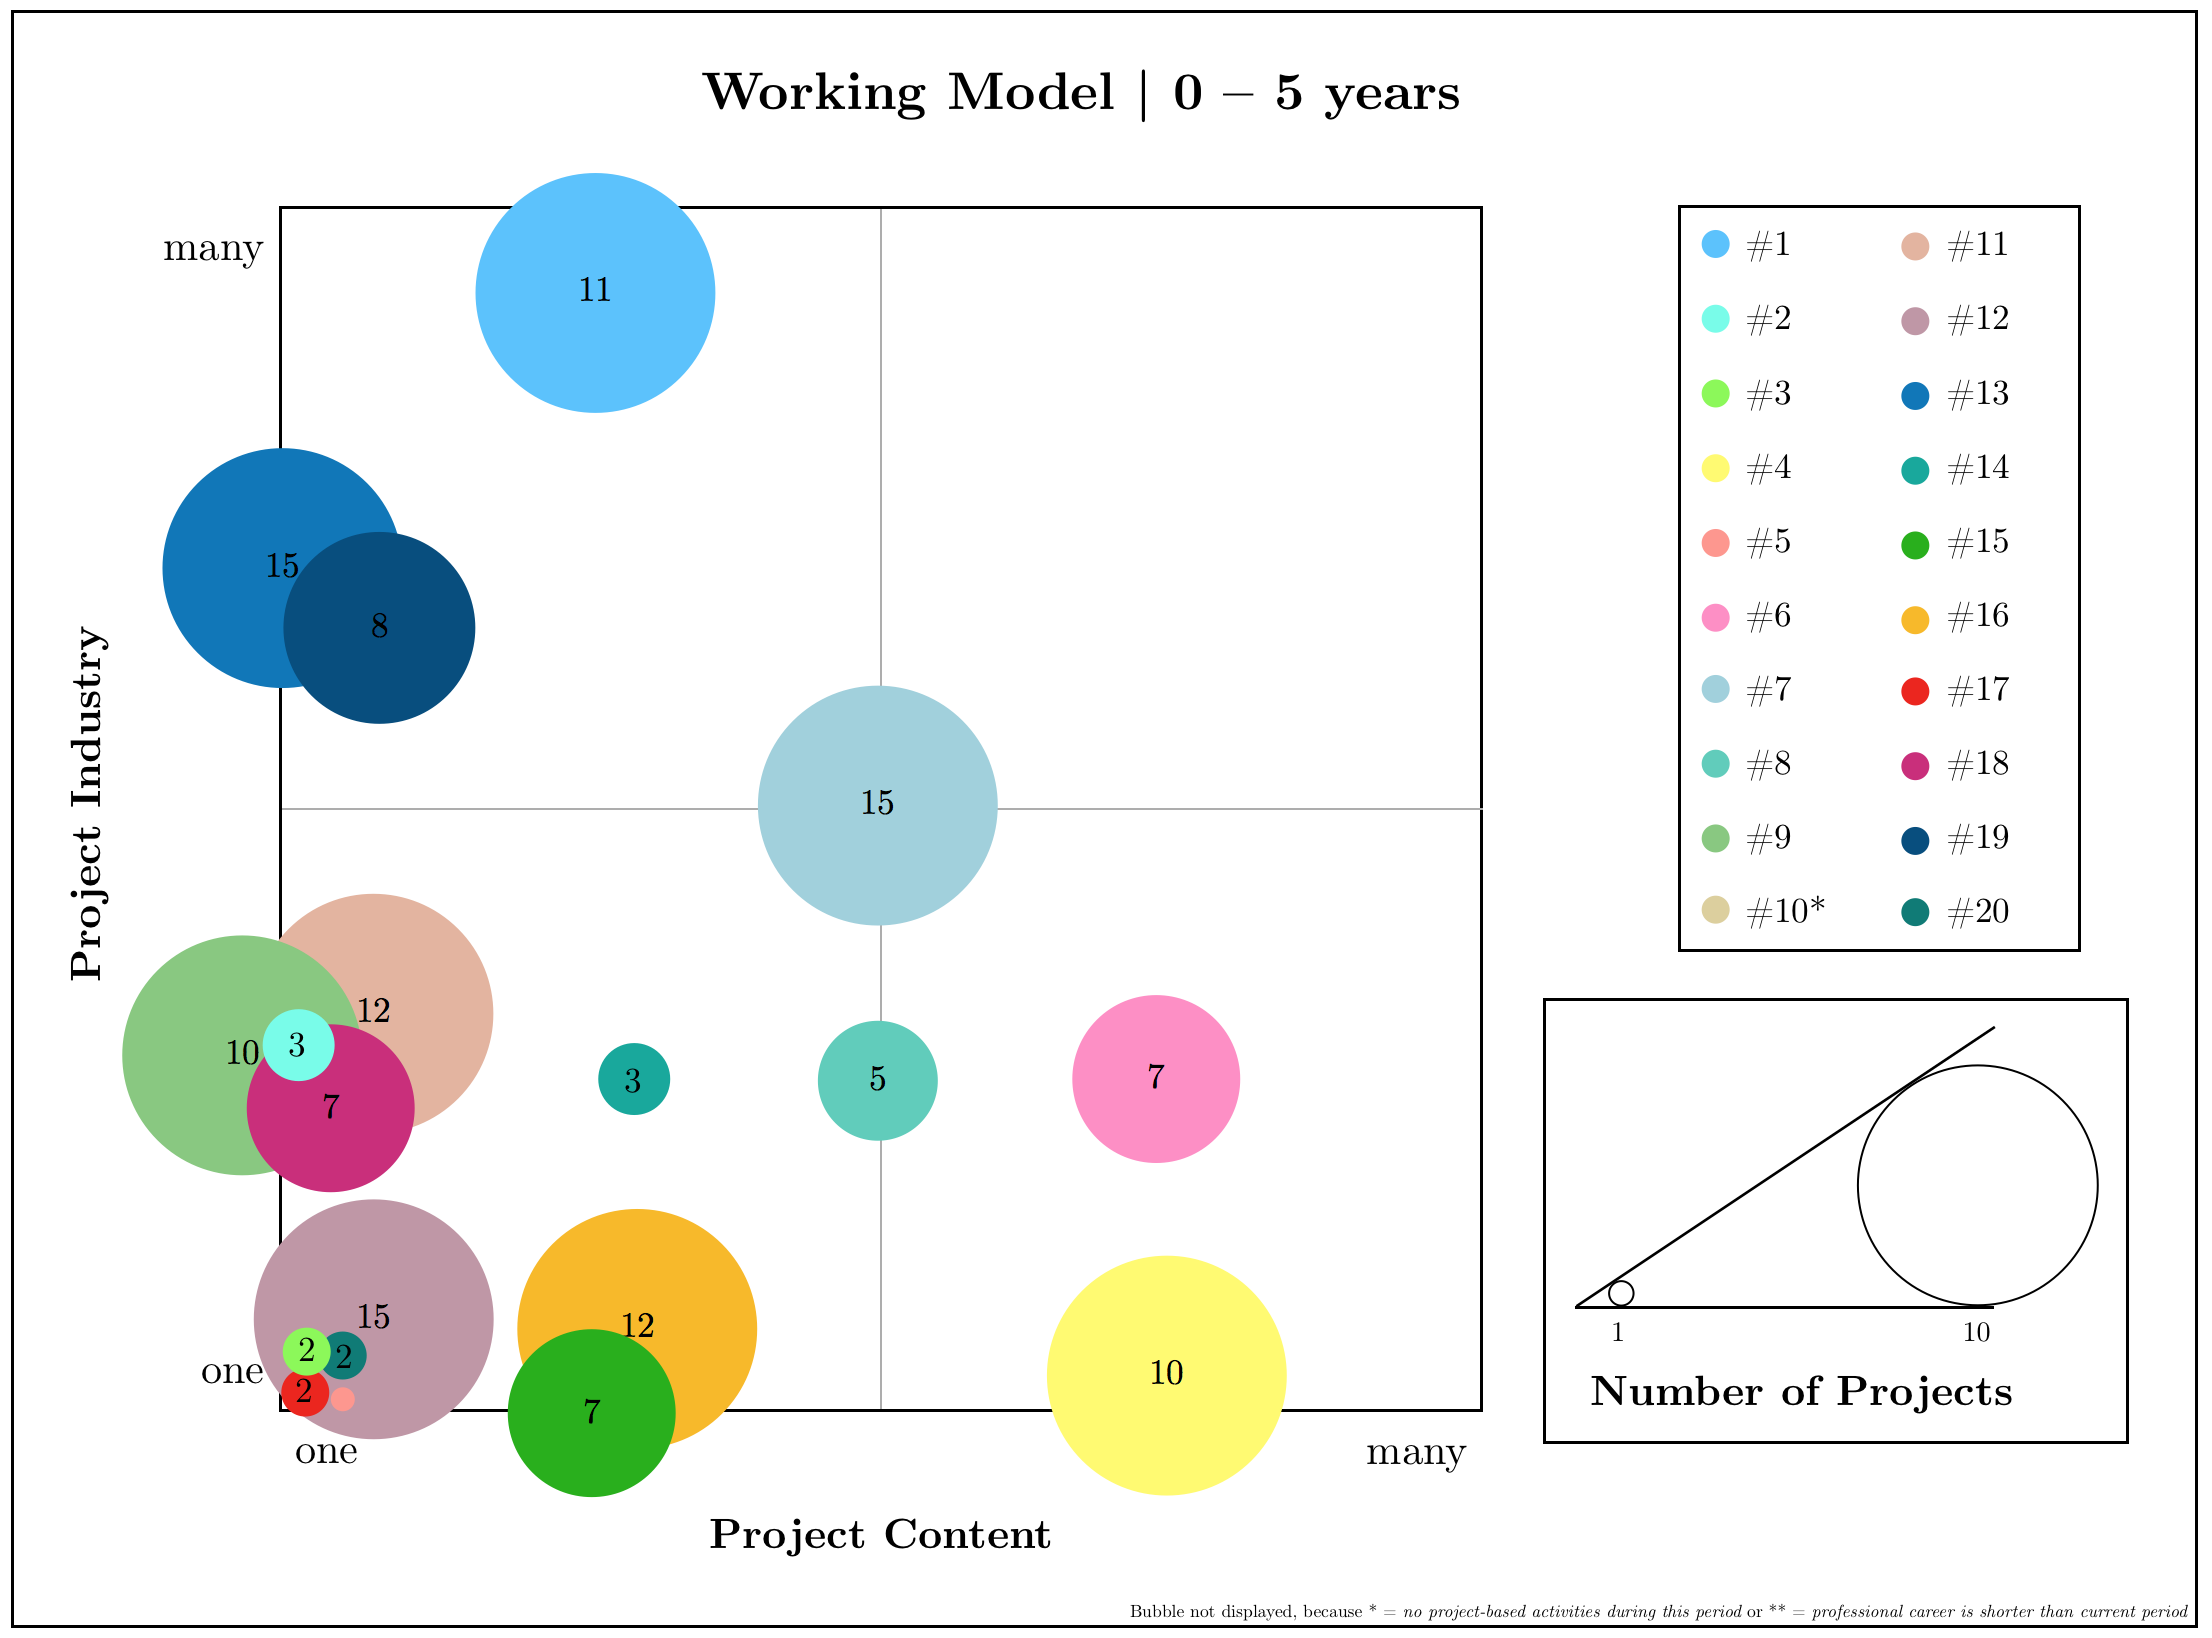
\includegraphics[width=0.75\columnwidth]{figures/WM_0005.png}
  \caption[Results of the working model: 0–5 years]{Results of the working model for the \nth{1} career period (0 – 5 years)}
  \label{fig:WM_0005}
  
\vspace*{.6cm}

\minipage[t]{0.48\textwidth}
  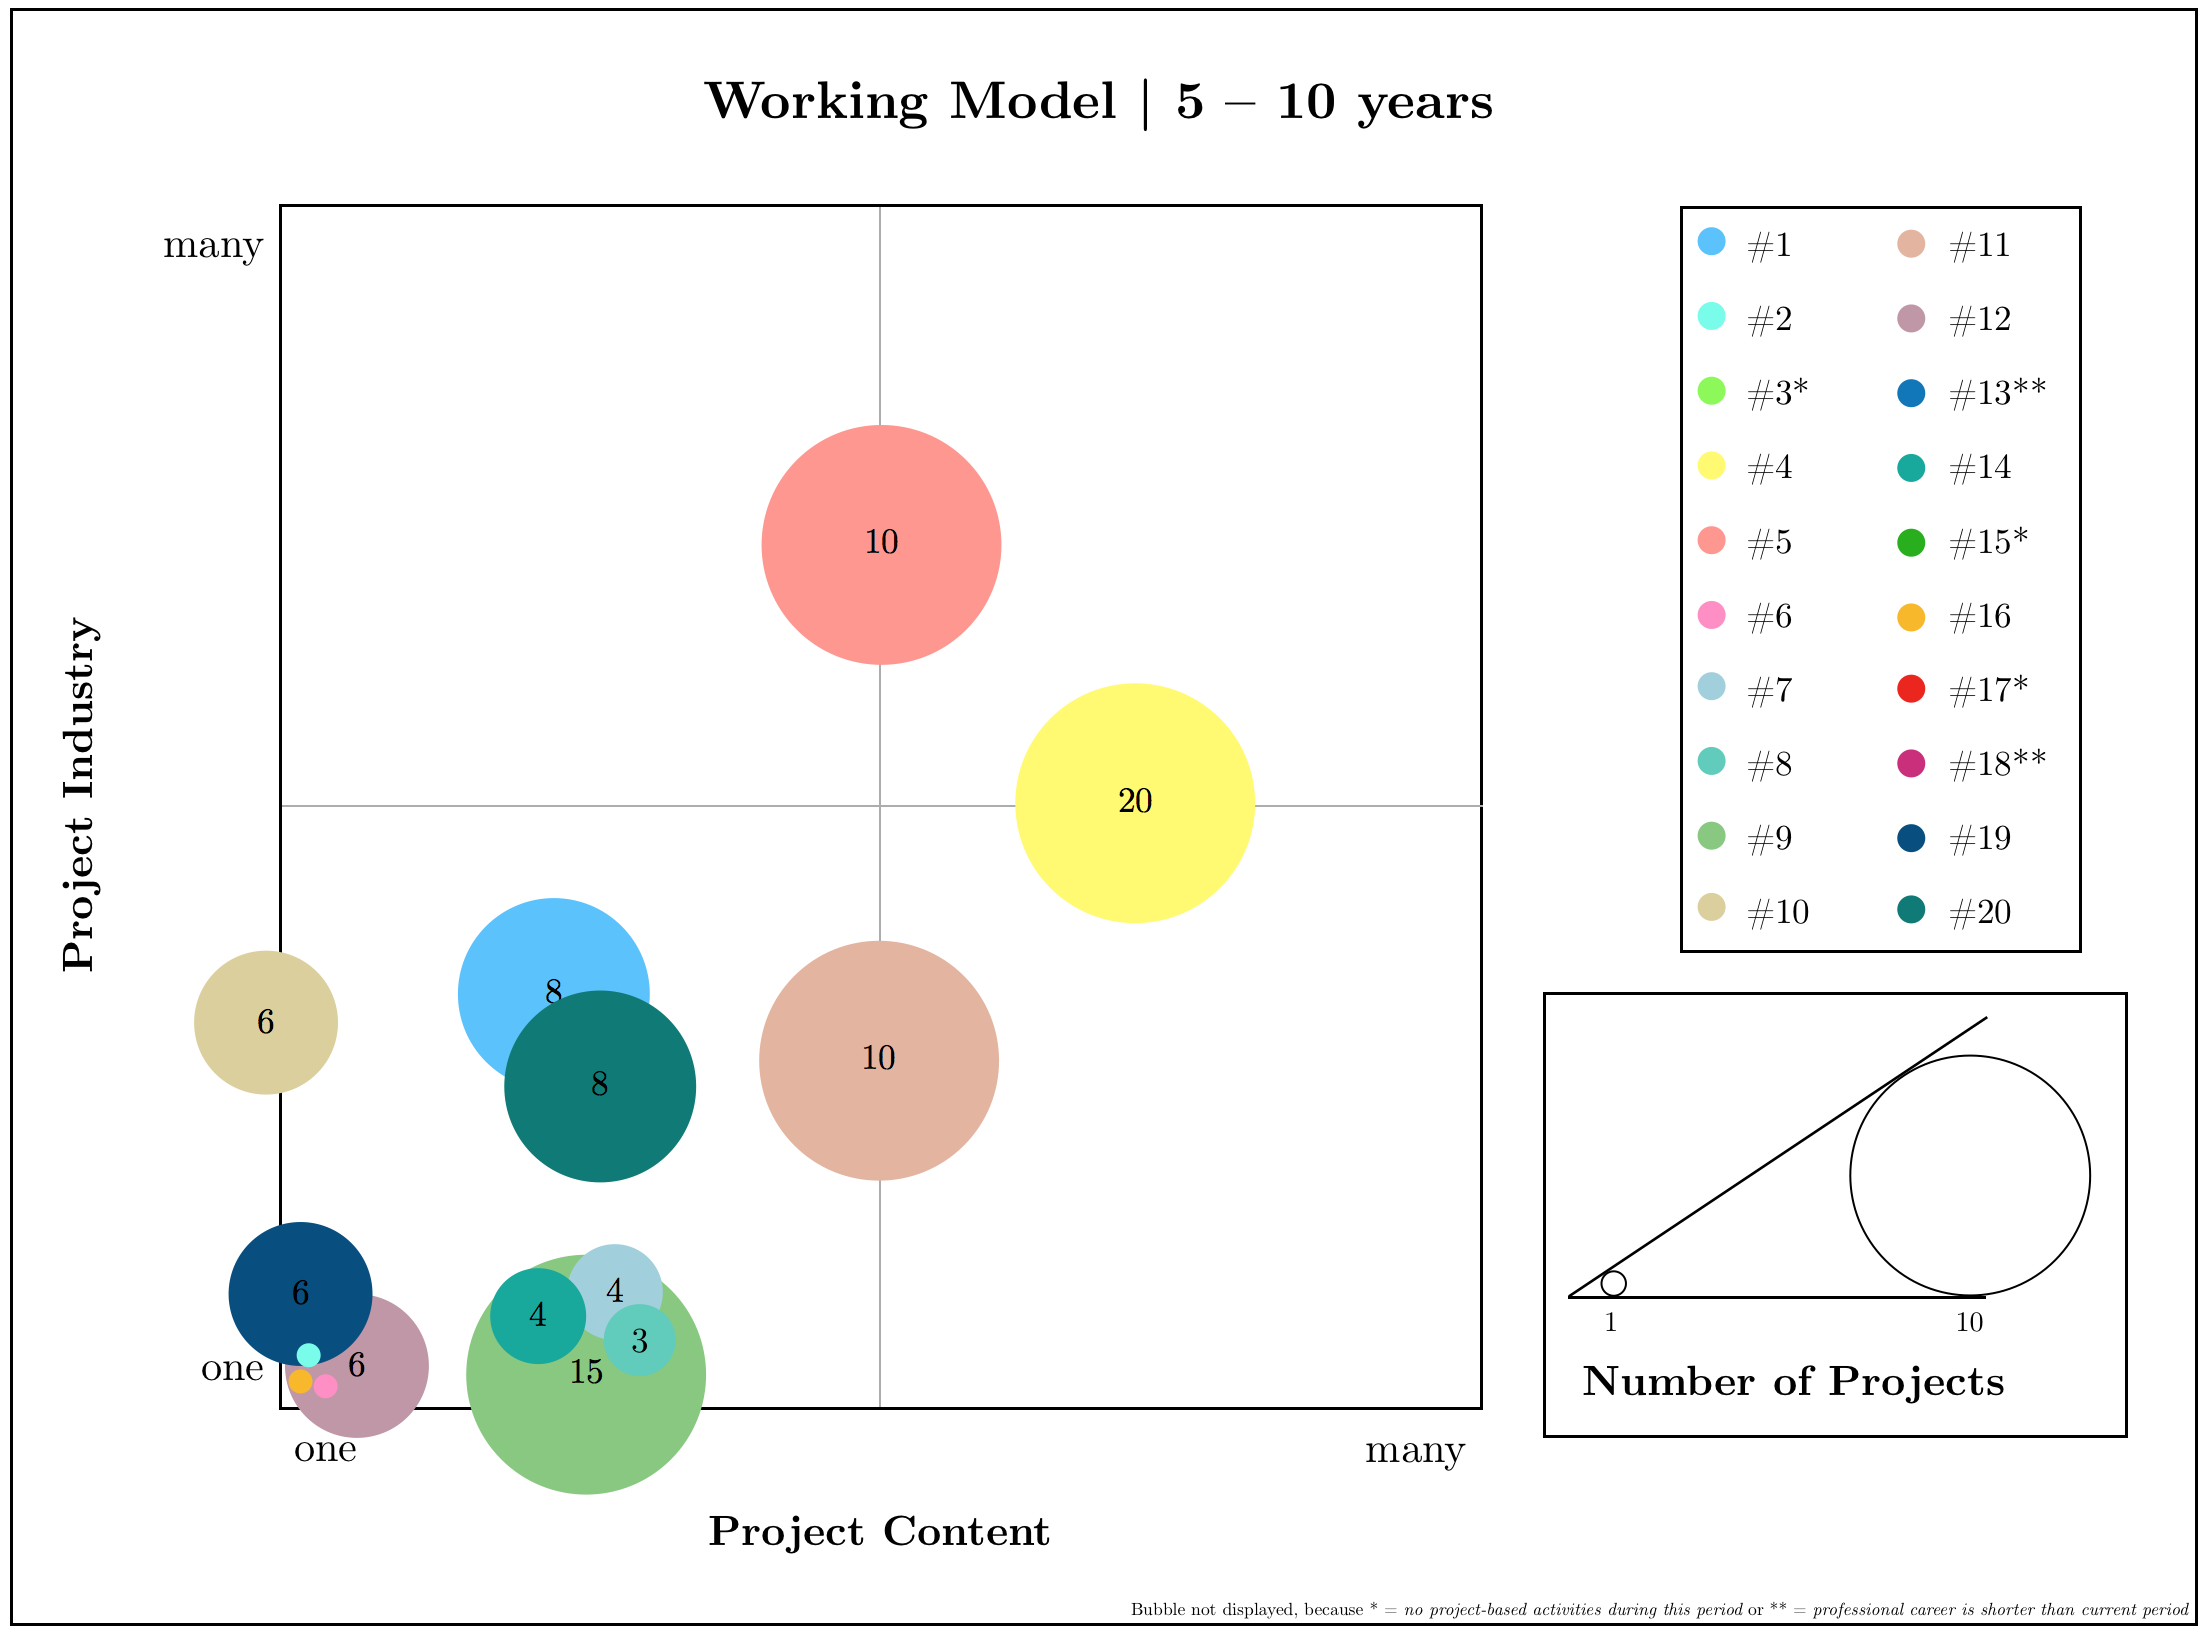
\includegraphics[width=\linewidth]{figures/WM_0510.png}
  \caption[Results of the working model: 5–10 years]{Results of the working model for the \nth{2} career period (5–10 years)}
  \label{fig:WM_0510}
\endminipage\hfill
\minipage[t]{0.48\textwidth}
  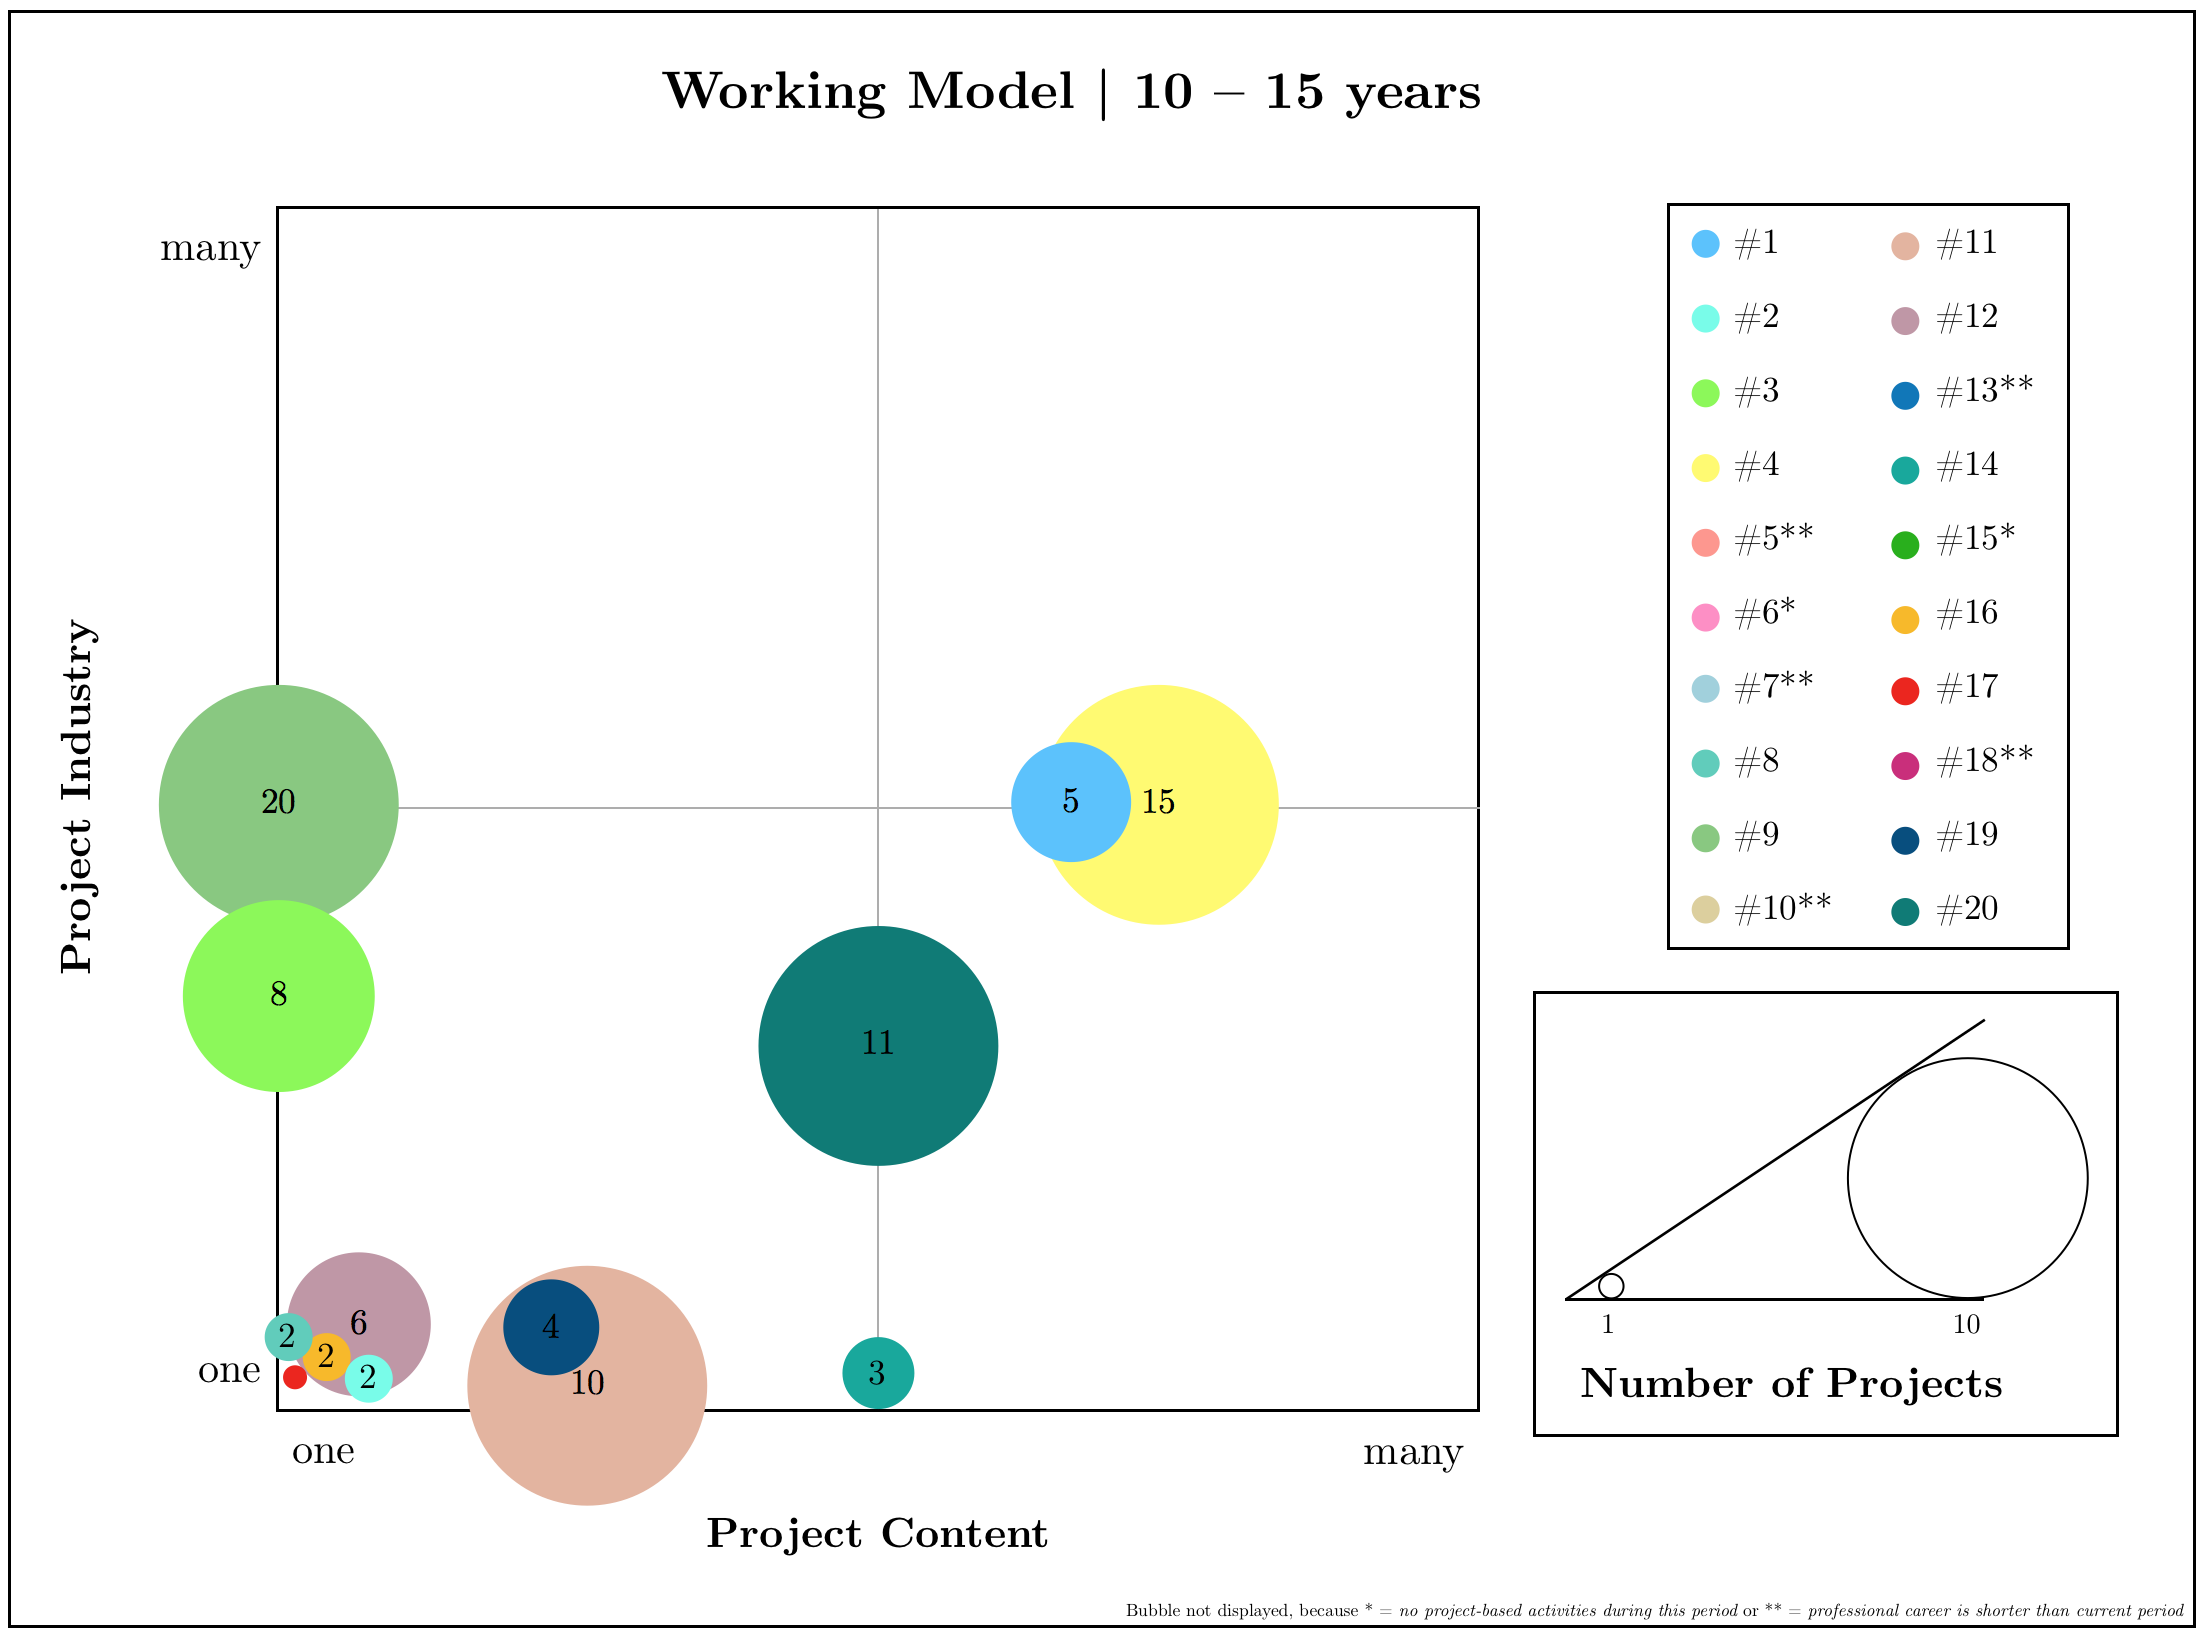
\includegraphics[width=\linewidth]{figures/WM_1015.png}
  \caption[Results of the working model: 10–15 years]{Results of the working model for the \nth{3} career period (10–15 years)}
  \label{fig:WM_1015}
  \endminipage

\vspace*{.6cm}

\minipage[t]{0.48\textwidth}
  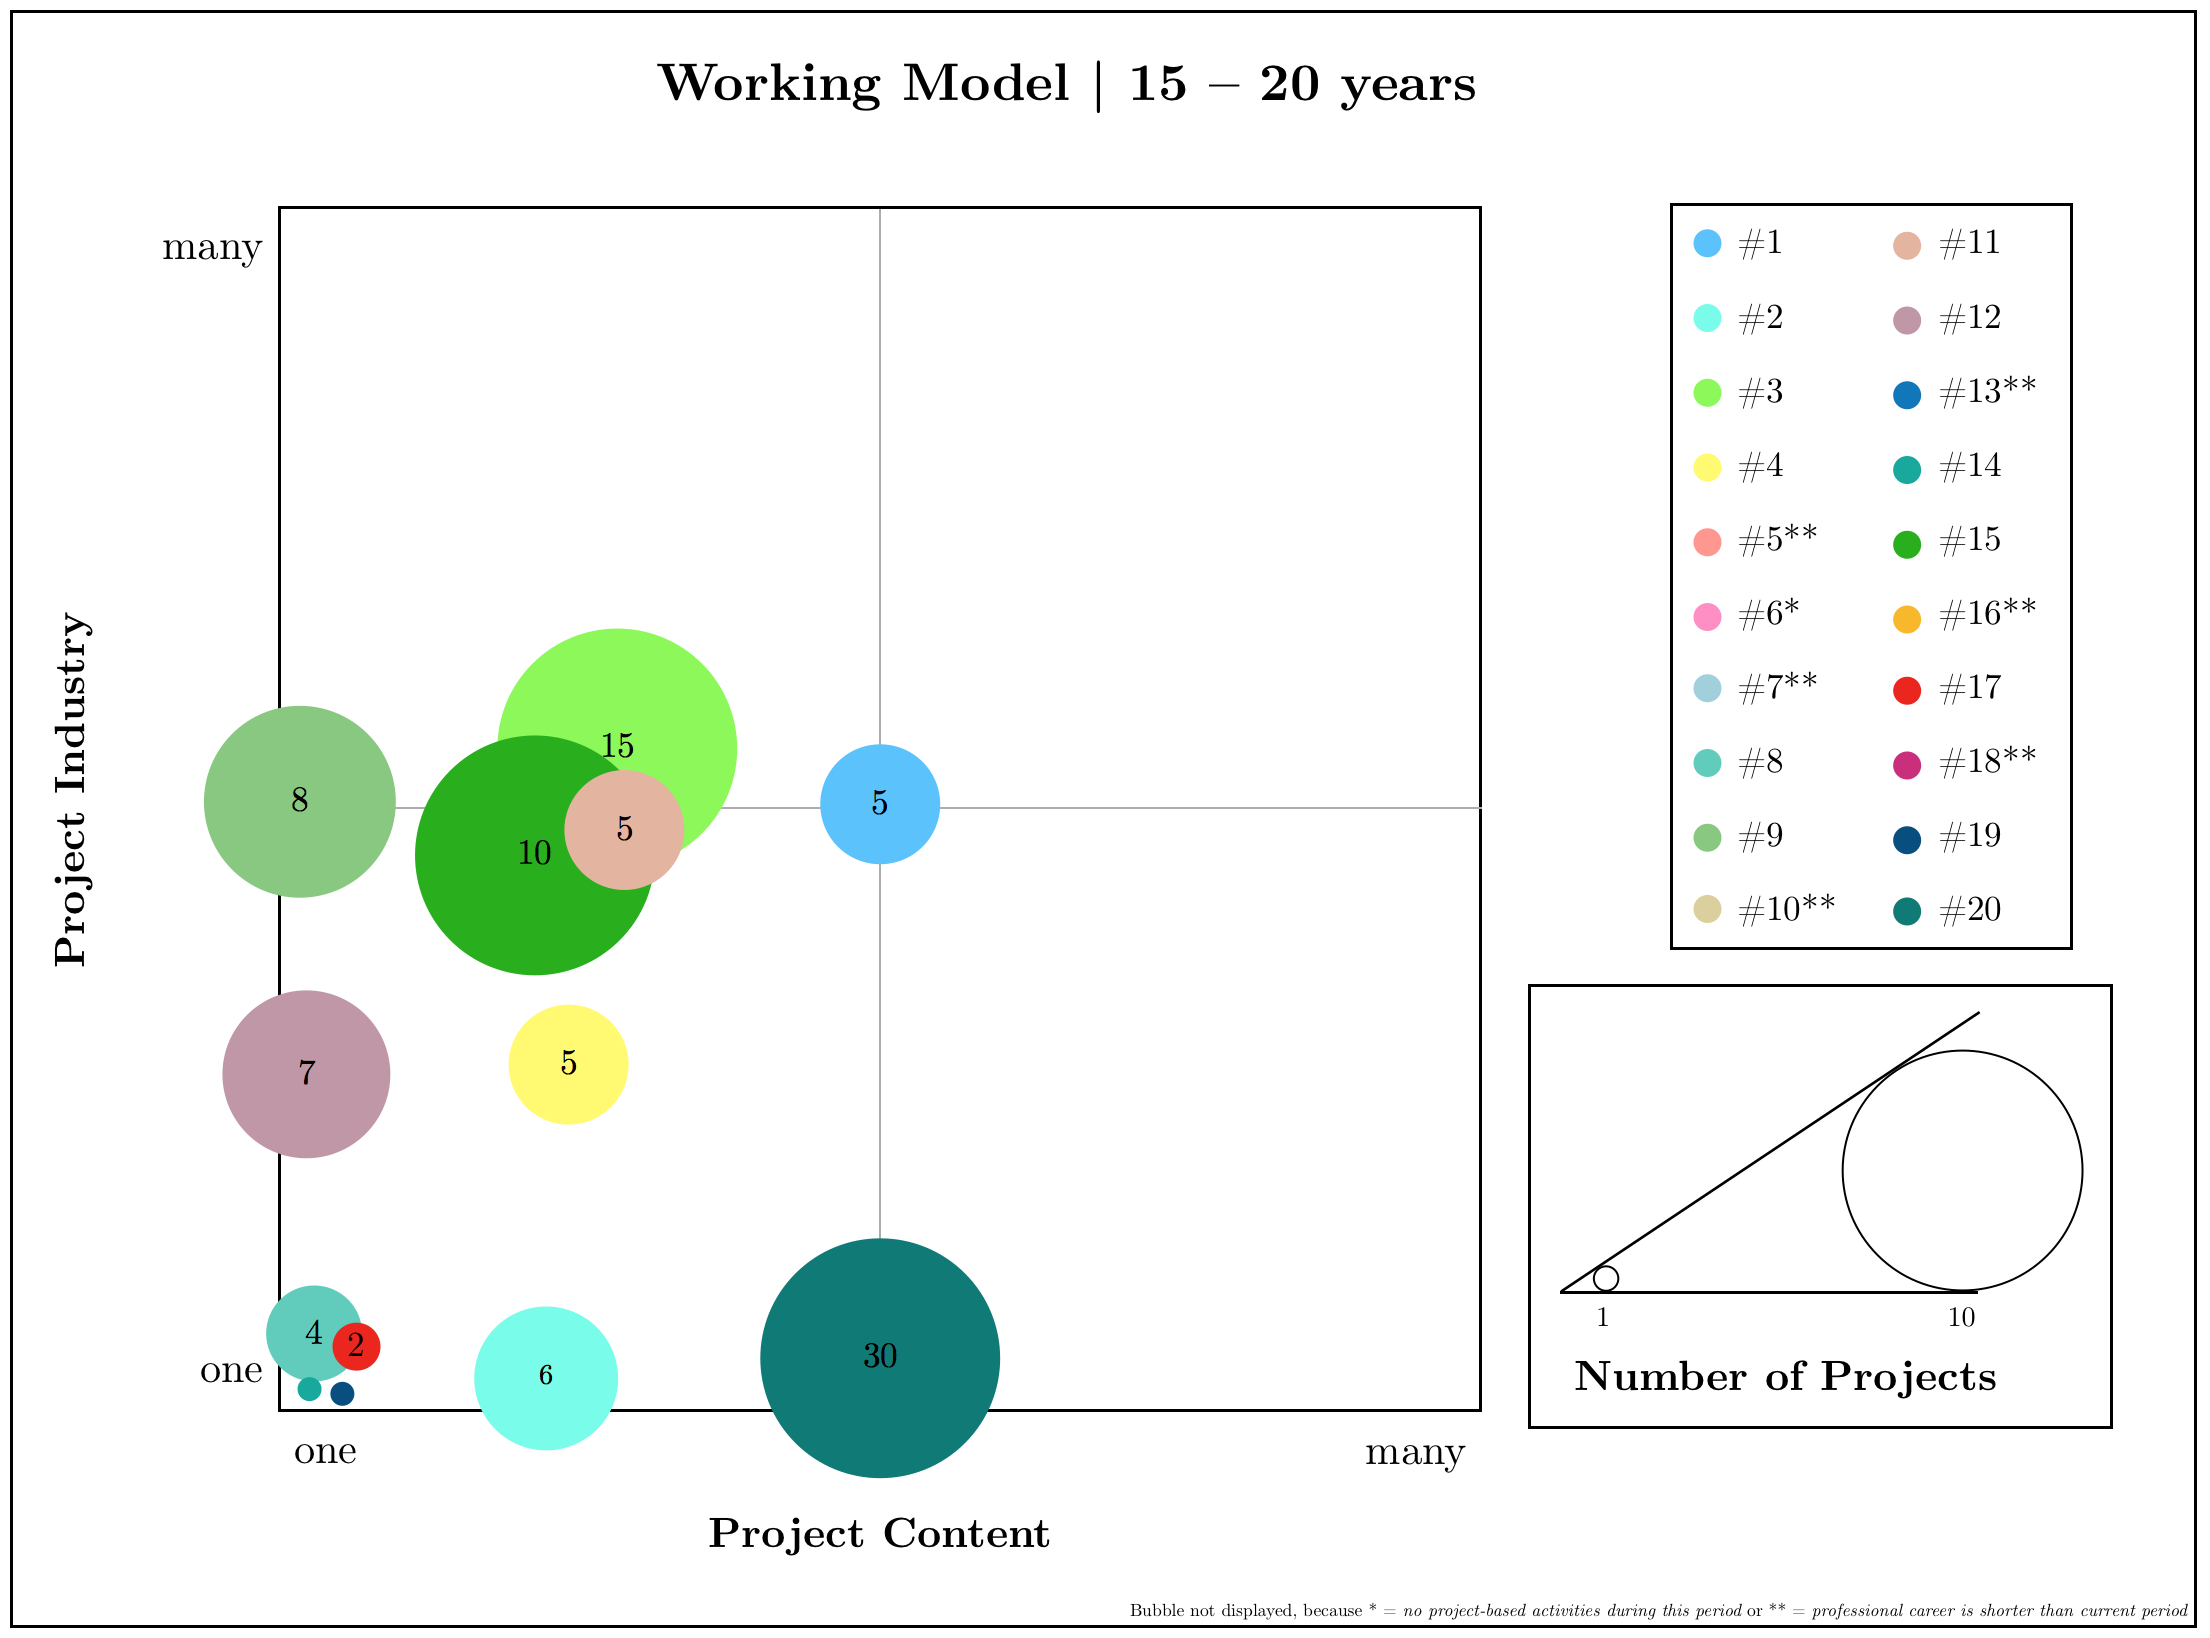
\includegraphics[width=\linewidth]{figures/WM_1520.png}
  \caption[Results of the working model: 15–20 years]{Results of the working model for the \nth{4} career period (15–20 years)}
  \label{fig:WM_1520}
\endminipage\hfill
\minipage[t]{0.48\textwidth}
  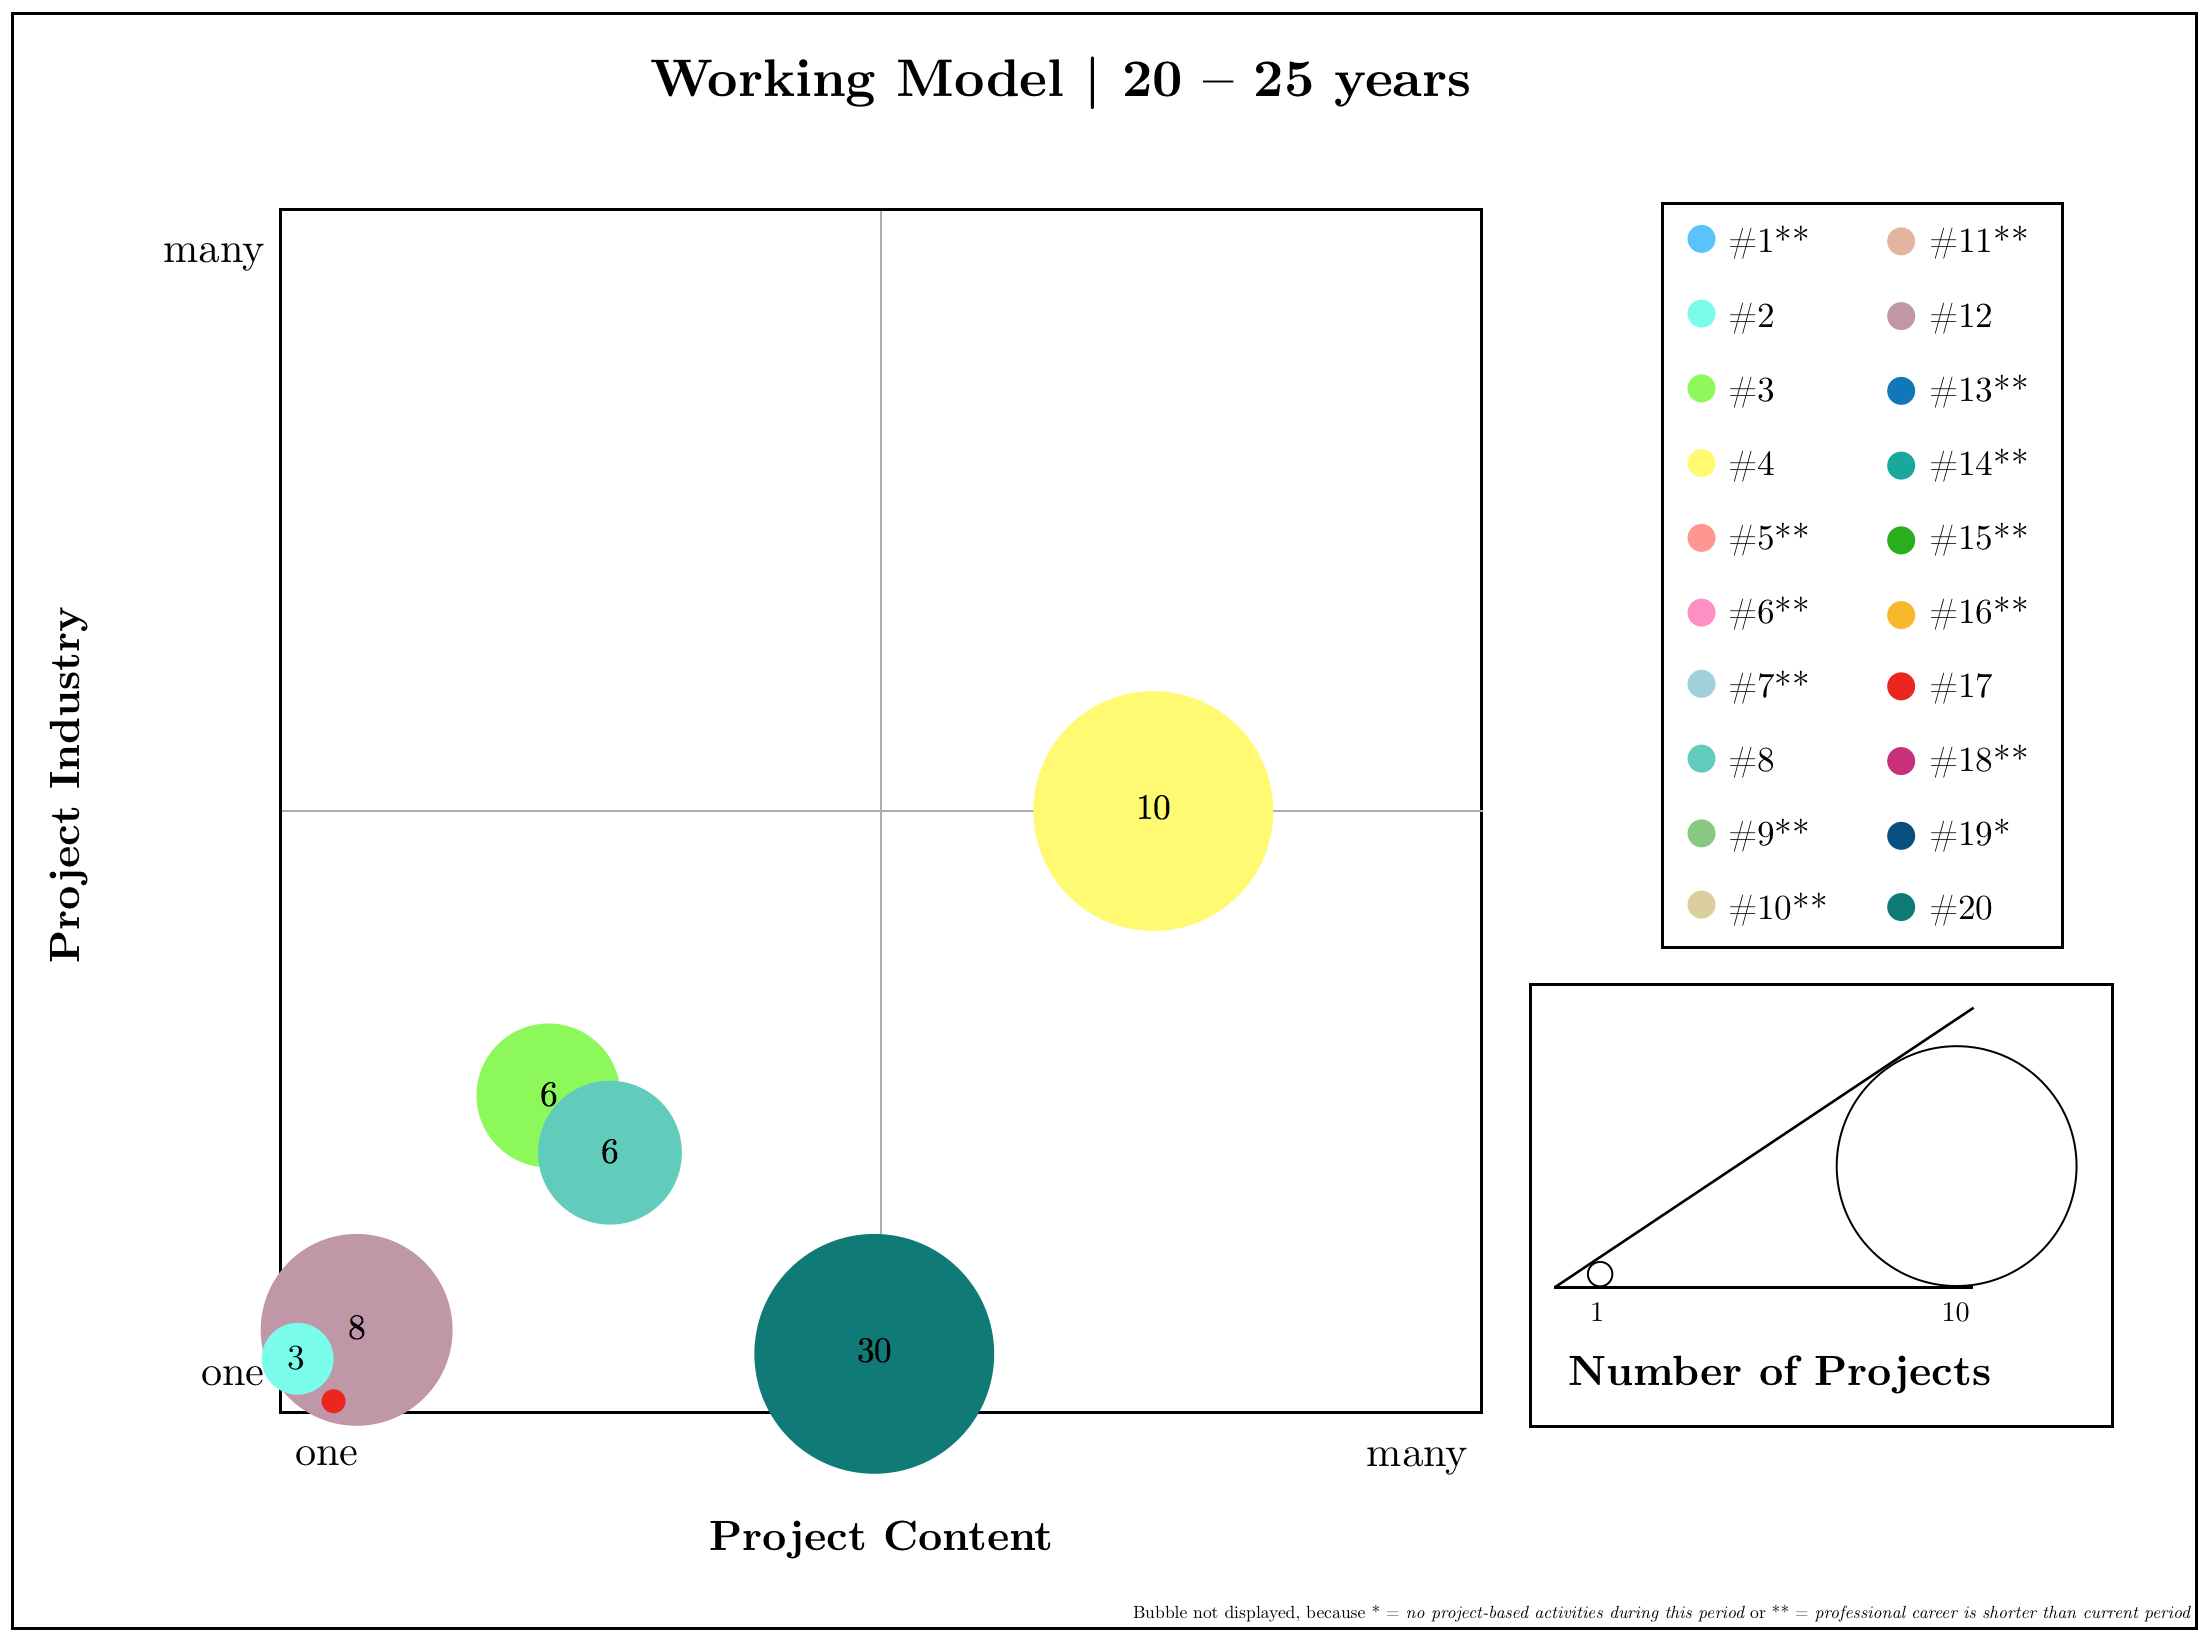
\includegraphics[width=\linewidth]{figures/WM_2025.png}
  \caption[Results of the working model: 20–25 years]{Results of the working model for the \nth{5} career period (20–25 years)}
  \label{fig:WM_2025}
  \endminipage
\end{figure}



%————————————————————–––––––Sub–Subsection–1————––––––––———————————————
%————————————————————Period-specific evaluations———————————————————

\noindent {\bf Period oriented analyses}\\[.1cm]
The first period-oriented analysis figure \ref{fig:analy_CC} (p. \pageref{fig:analy_CC}) analyses the number of company changes per project professional for every time period of his/her career. The basis (total number of project professionals), decreases from period to period as the majority of the interviewees have a professional experience shorter than 25 years, which is also relevant for the following analyses in this subsection (Basis for each period: \nth{1} period: 20 PP; \nth{2} period: 18 PP; \nth{3} period: 15 PP; \nth{4} period: 14 PP; \nth{5} period: 8 PP;). As the this thesis tries to find patterns in the careers of project professionals, this could be a helpful indicator during the analysis. Besides the evaluation of this perspective for the entire sample group, it was also also conducted for each a 'younger' and an 'older' subgroup, which was split according to the  mean age value of 47 years. This additional perspective was taken in order to see if there a significant difference between these two age groups regarding company changes. As the blue line in figure \ref{fig:analy_CC} shows, the number of company changes per project professional decreases over the course of the career, as is falls from 0.60 company changes per PP in the first period to 0.13 in the last one. Furthermore, a difference is evident between the two age groups over the course of their career. In the first two periods the younger subgroup has an elevated level of company changes of 0.75  and 0.67 company changes per PP. However then the rate falls to 0.33 in the \nth{3} period, before rising again drastically to 1 company  change per PP. In contrast, the older subgroup has a lower rate of each time 0.5 in the first two periods, but then increases and outstrips the rate of the other subgroup with a rate of 0.58, before decreasing again drastically in the last two periods to 0.25 and 0.13 company changes per PP.  \\

\begin{figure}[!hbt]
    \captionsetup{font=small}
  \centering
  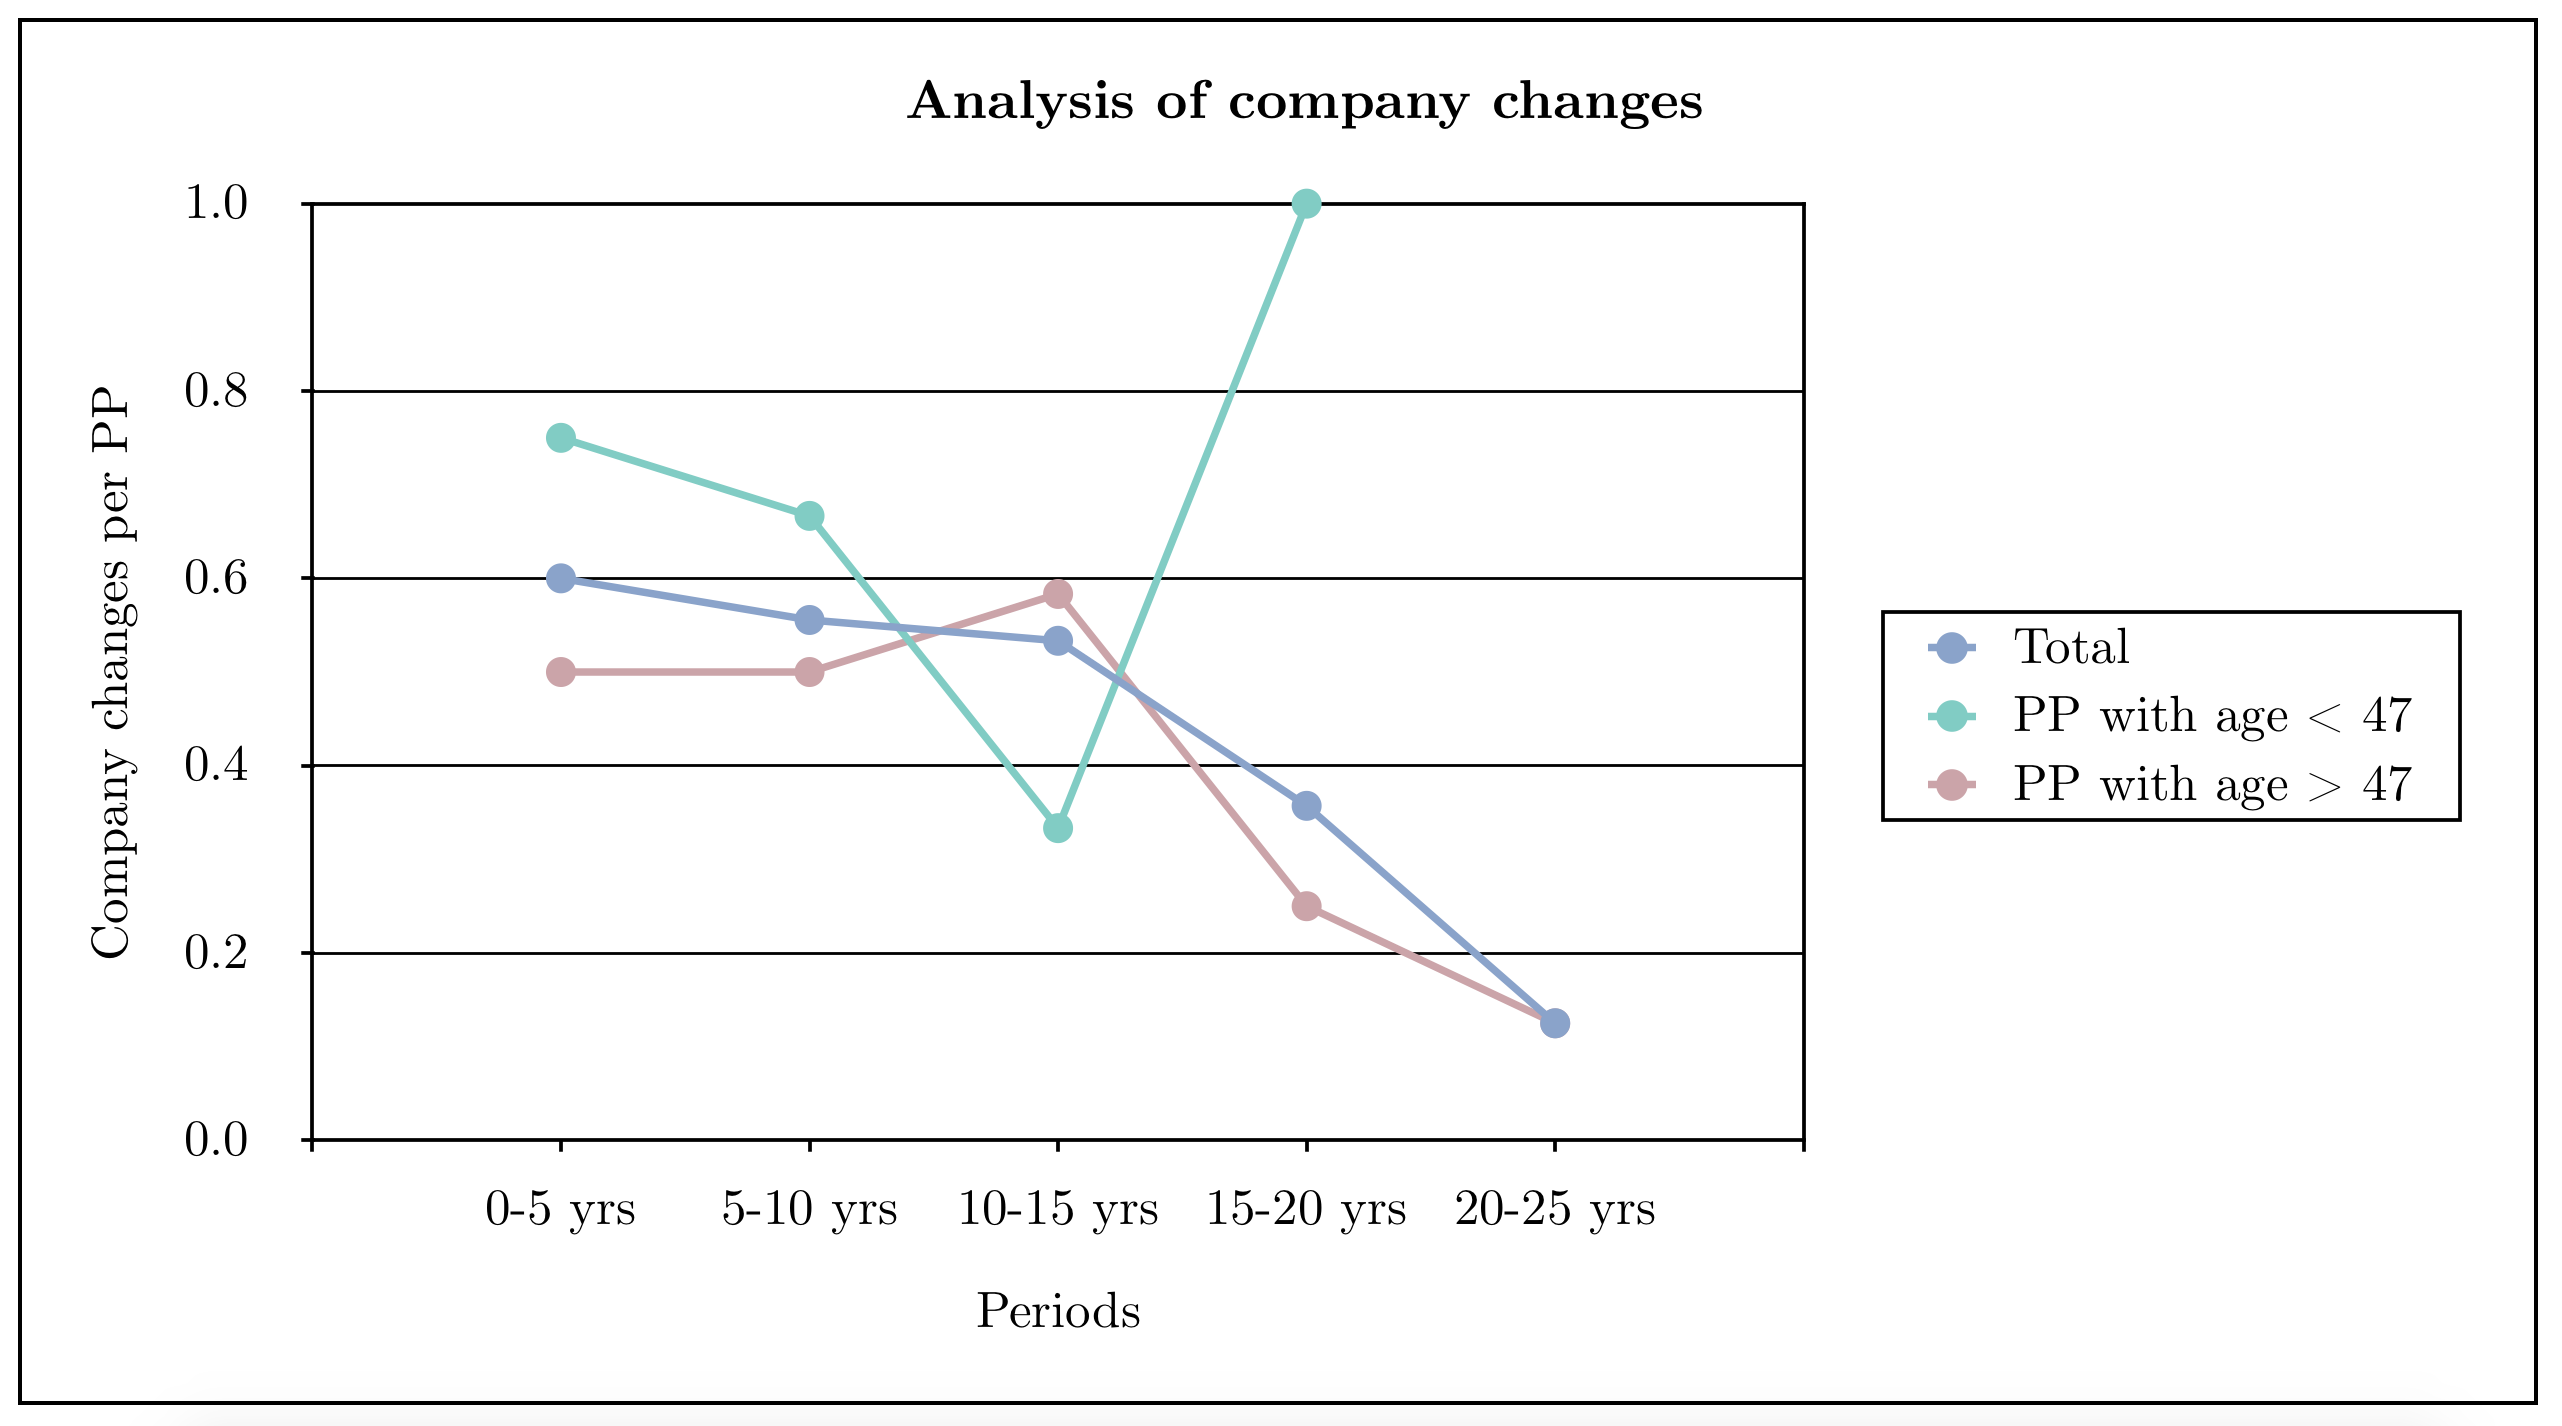
\includegraphics[width=.6\columnwidth]{figures/Analysis_CC.png}
  \caption[Analysis of company changes]{Analysis of company changes per candidate for each career period. The results are shown not only for the entire sample, but also the younger and older half of it (divided by the mean age 47).}
  \label{fig:analy_CC}
\end{figure}


Figure \ref{fig:analy_PCI} (p. \pageref{fig:analy_PCI}) and figure \ref{fig:analy_NP} (p. \pageref{fig:analy_NP}) take a similar perspective as they both evaluate two or one, respectively, of the three dimensions of the main working model and set them into relation to active project professionals and each of the periods. Hereof, active project professionals refer to those those project professionals, who did project-based work in the corresponding period.

The first of the two figures, figure \ref{fig:analy_PCI}, depicts the results of the evaluation of in how many project contents and industries the active project professionals worked in each of the periods on average. Thereby it gives an insight into the distribution of the two indicators over the project professional's career. The results show respectively  project industries that in the \nth{1} career period projects in the most project industries are conducted (2 per active PP). In the \nth{4} period an almost as high value is reached with 1.92 per active PP. In the other three time periods values of between 1.57 and 1.62 project industries per active PP are evident. With respect to the second dimension depicted in figure \ref{fig:analy_PCI}, project contents, it showcases a lower number of project contents per active PP of 1.74 in the first period. In the following two periods the average number of project contents worked in overtakes the avergae number of project industries, with values of 1.87 and 1.92, before falling to the lowest value of the entire depicted time span  of 1.69 per active PP. In the last period of their career an average of 2 project contents per active PP were worked in.  \\

\begin{figure}[!hbt]
    \captionsetup{font=small}
  \centering
  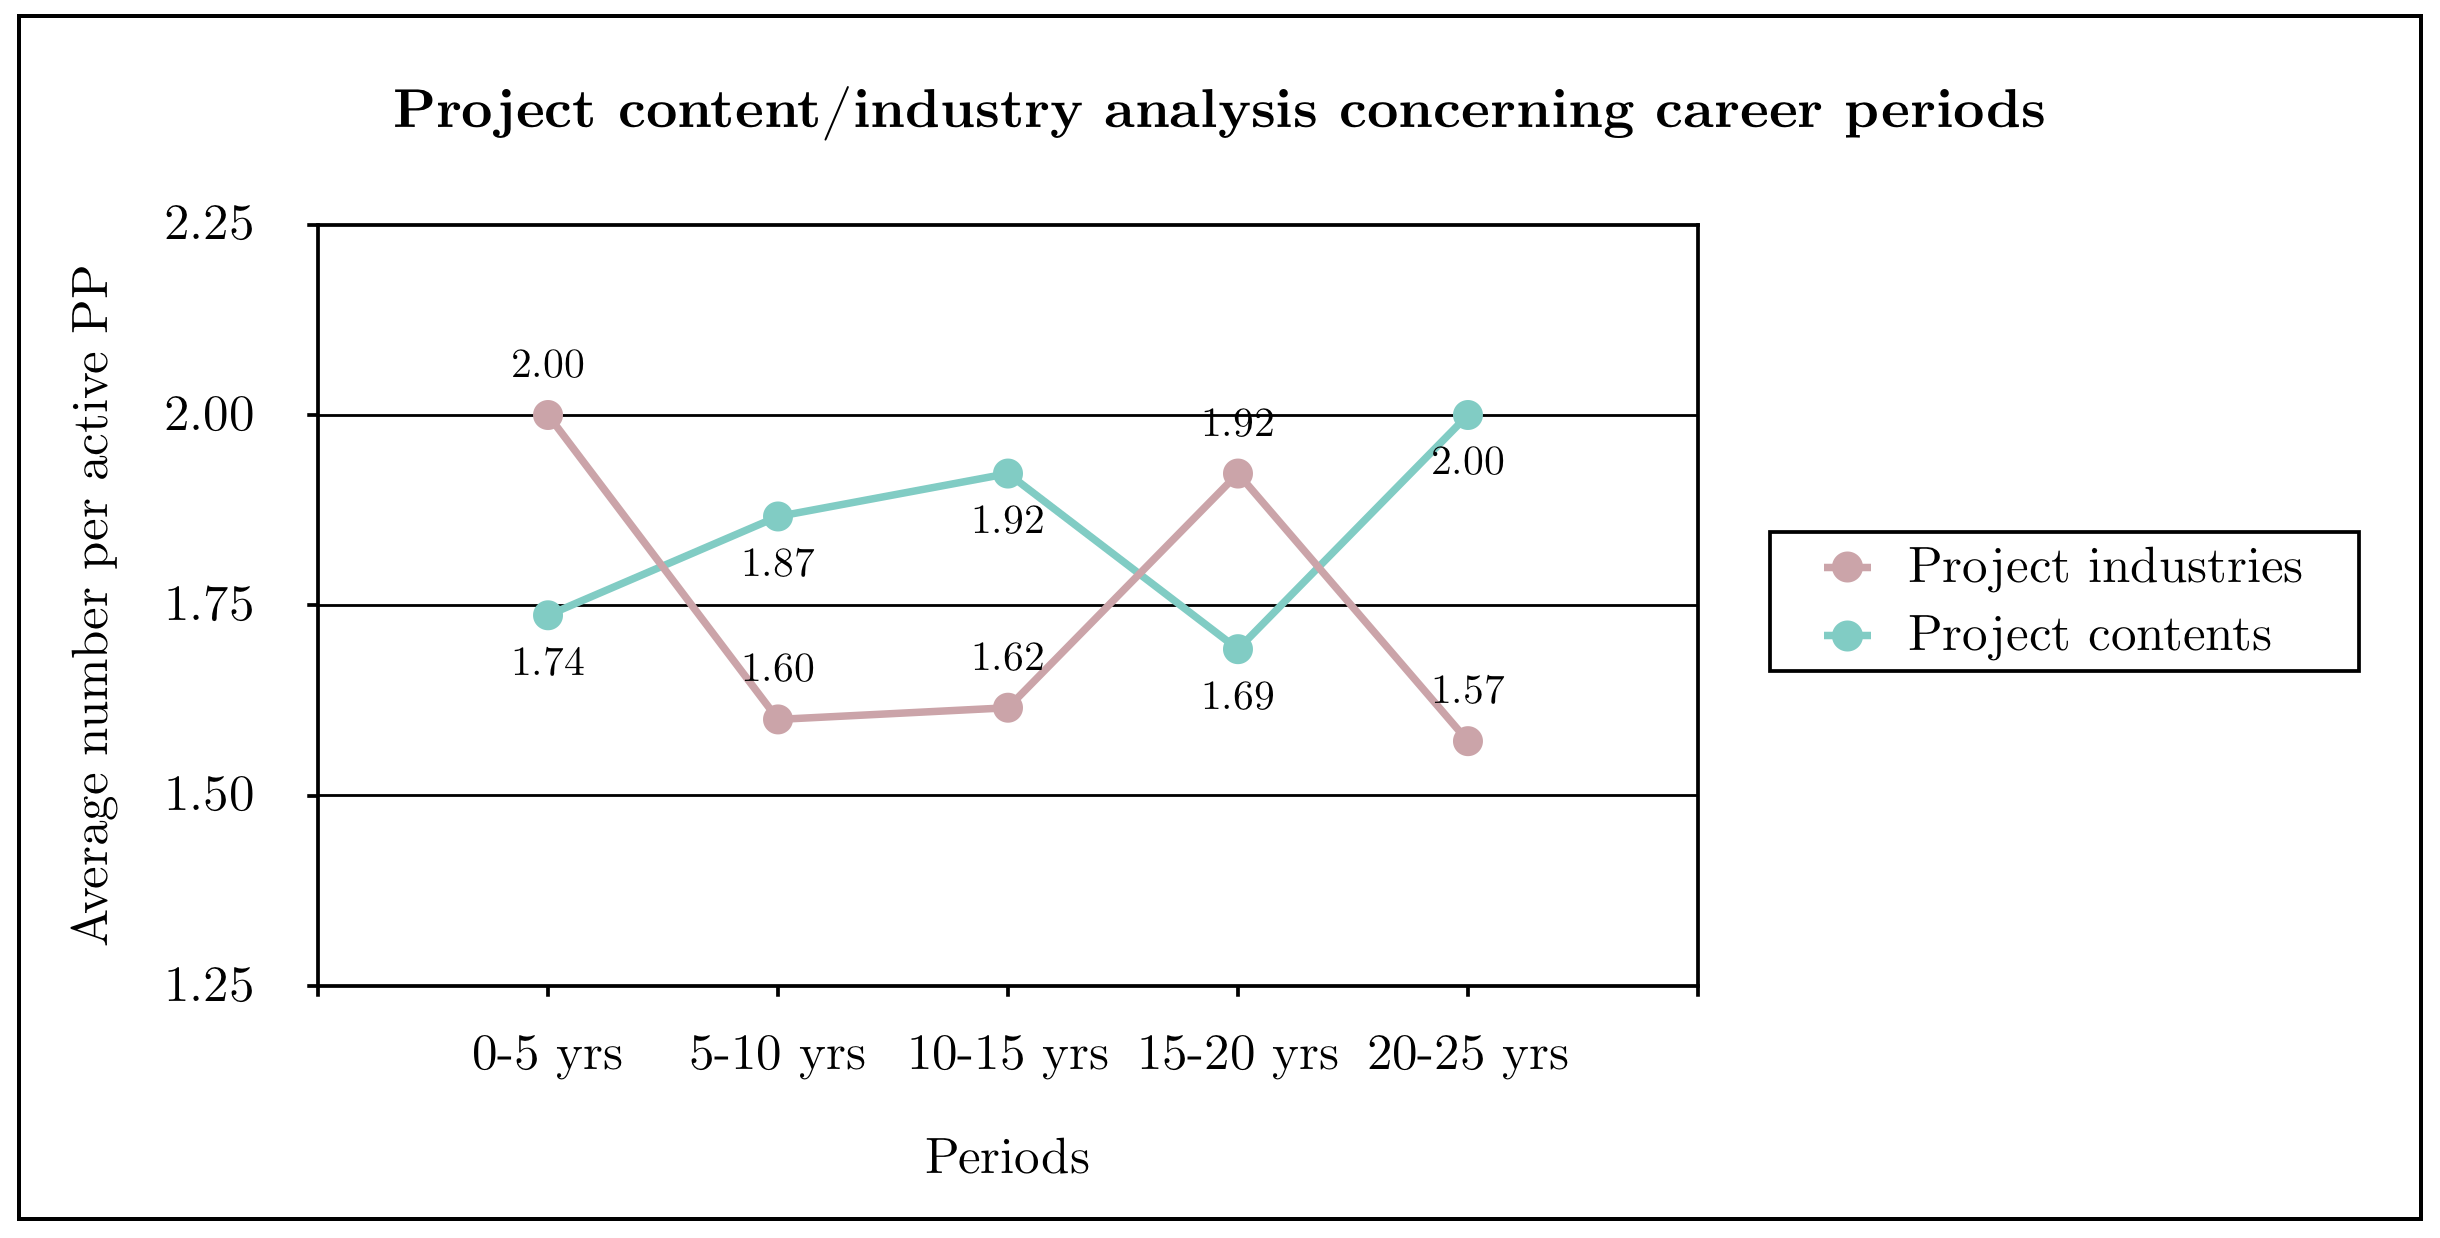
\includegraphics[width=.6\columnwidth]{figures/Analysis_PCI.png}
  \caption[Analysis of project contents and industries respectively the PP's career]{Analysis of the average number of project contents and industries respectively each period of the project professional's career}
  \label{fig:analy_PCI}
\end{figure}

The second figure, figure \ref{fig:analy_NP}, analyses the average number of projects conducted per active project professional for each of the five career periods. It helps, as the before presented figure, to get a feeling for how the average number of projects conducted is distributed over the sample group's career. The results show that the number of projects conducted is elevated (7.74) in the \nth{1} period, in comparison to the \nth{2} and \nth{3} period, where the value is relatively stable at about 1.6 projects contents per active PP. However, in the last two terms it rises drastically to 7.62 and 9.14 per active PP, respectively.\\


\begin{figure}[!hbt]
    \captionsetup{font=small}
  \centering
  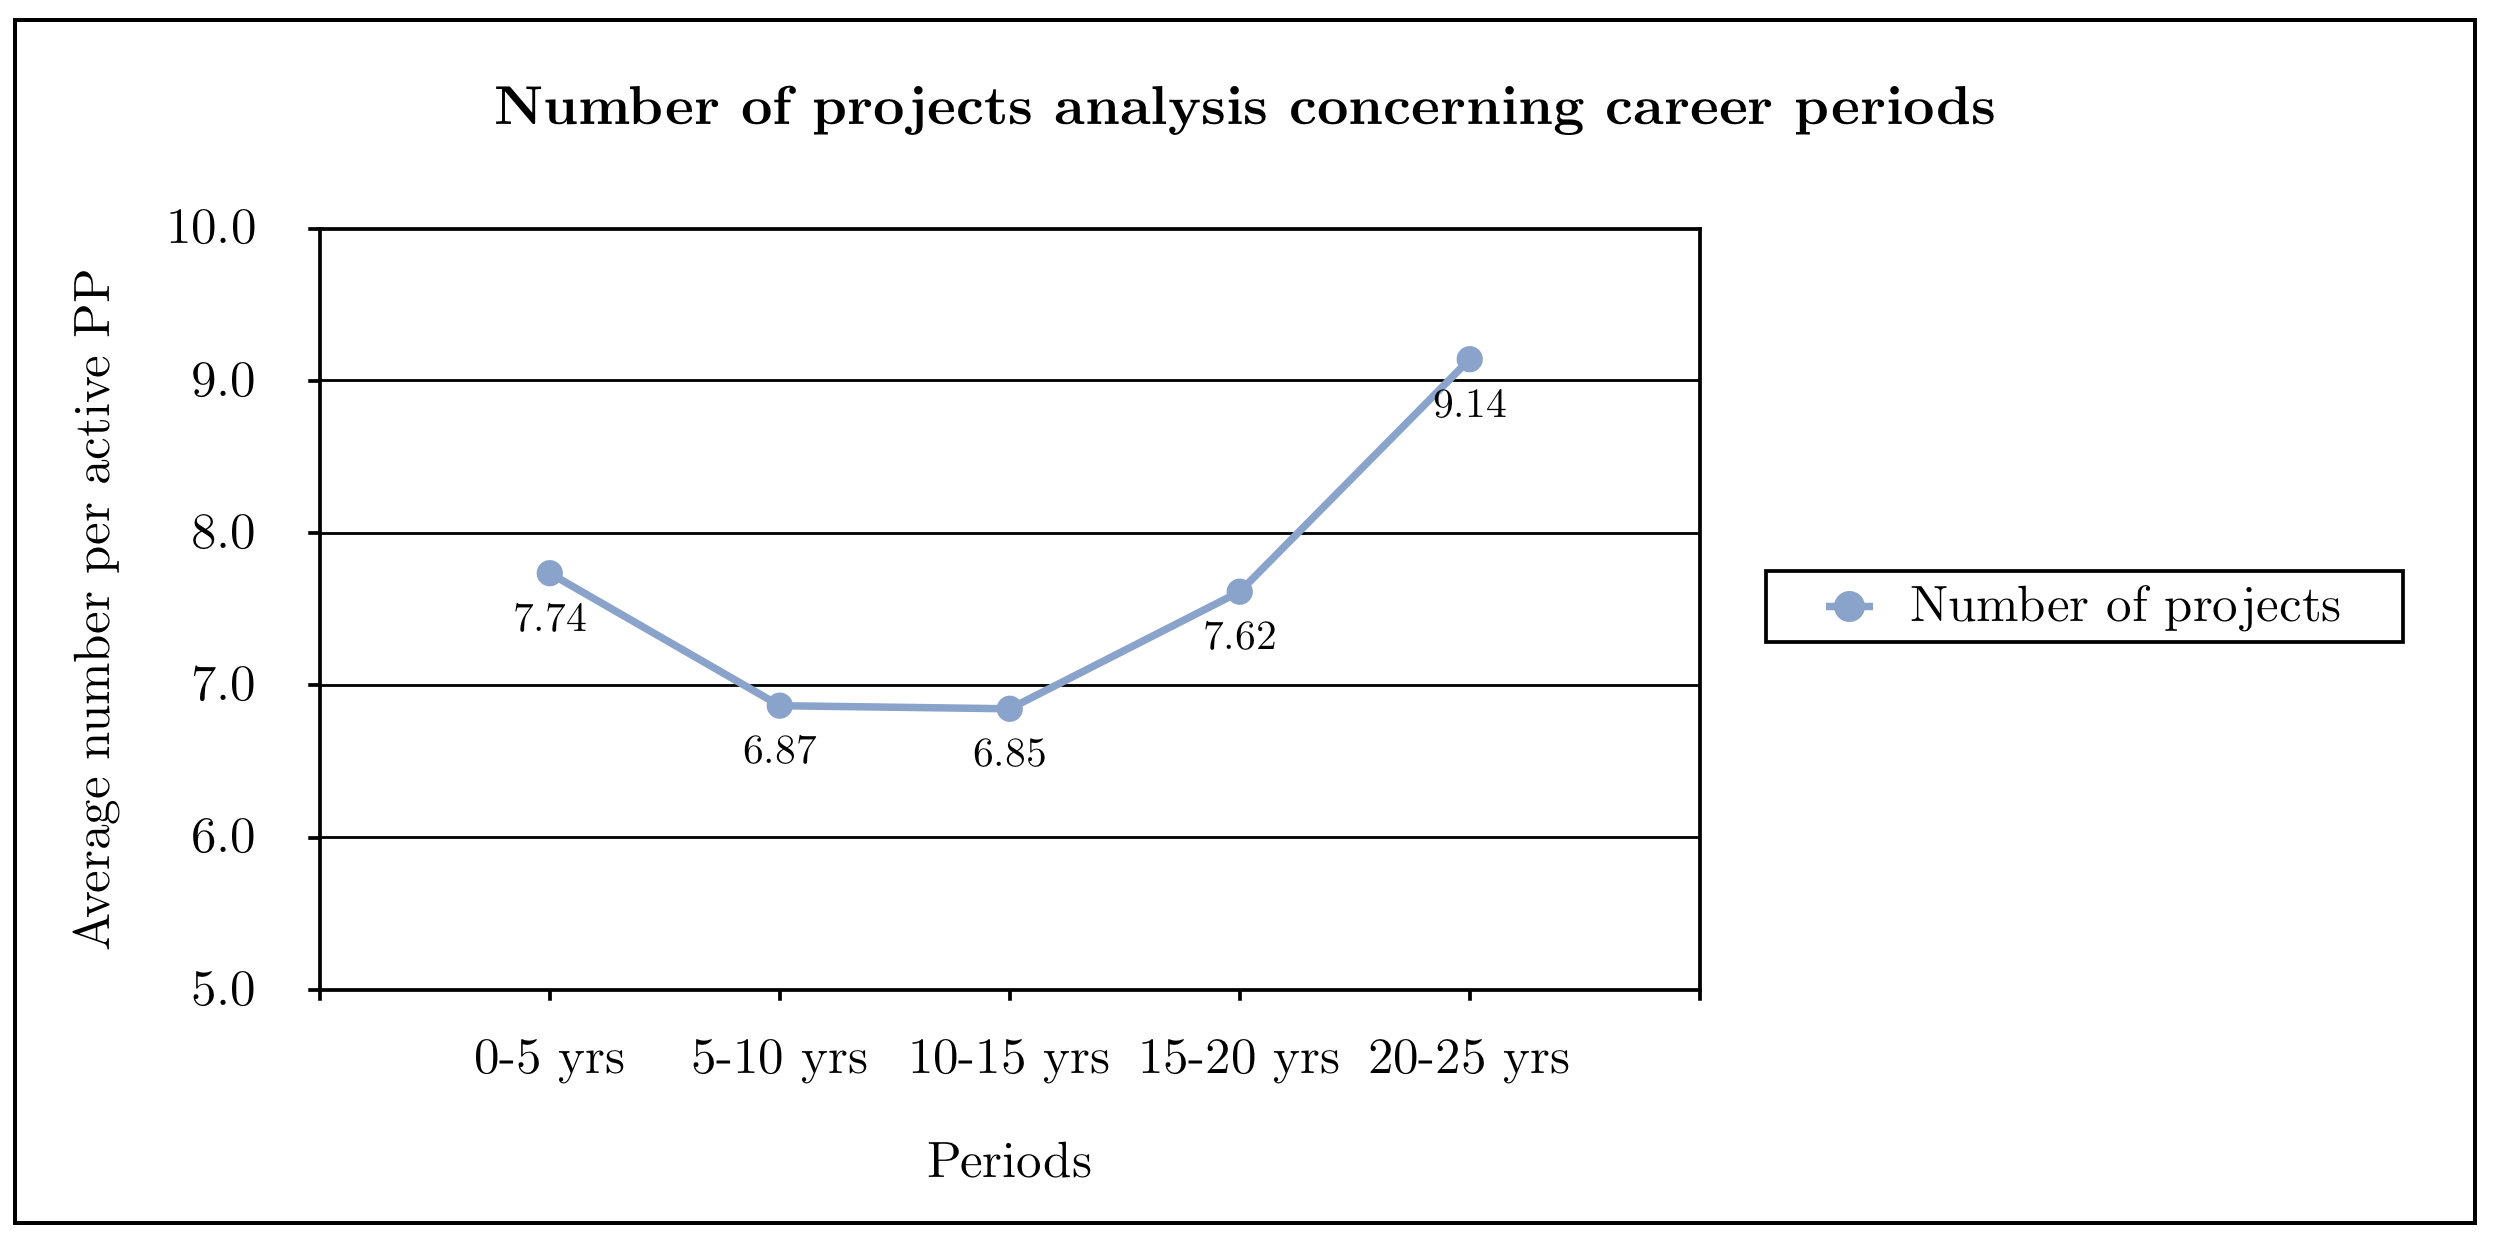
\includegraphics[width=.6\columnwidth]{figures/Analysis_NP.png}
  \caption[Analysis of the number of projects respectively the PP's career]{Analysis of the average number of projects respectively each period of the project professional's career.}
  \label{fig:analy_NP}
\end{figure}



%————————————————Project–content/industry–evaluations———————————————

\noindent {\bf Project oriented analyses}\\[.1cm]
The analyses presented in this part are aimed at examining which project contents and industries were conducted the most in the total 67 five year-periods and if these correspond the distribution of industry backgrounds of the interviewees.

The first table, table \ref{tab:studycont} 
(p. \pageref{tab:studycont}), illustrates all possible project contents and the corresponding quantity they were identified in the data sets. The results show that the most found project contents were \textit{IT projects} (44), \textit{Organisational development projects} (24), \textit{Investment projects} (15), \textit{Strategy projects} (12) and \textit{Feasibility studies, Planning projects} (11). Furthermore, it can be derived that all of the 11 different project contents were at least found once.\\



\begin{table}[!hbt]
\centering
\captionsetup{font=small}
\footnotesize
    \begin{tabular}{|l|l|}
    \hline
    Project Content                                             & Quantity \\ \hline
    IT projects                                                 & 44       \\
    Organisational development projects                         & 24       \\
    Investment projects (construction, plant engineering, etc.) & 15       \\
    Strategy projects                                           & 12       \\
    Feasibility studies, planning projects                      & 11       \\
    Marketing projects, event projects                          & 6        \\
    Research projects, product development projects             & 5        \\
    Company participation projects                              & 2        \\
    Maintenance projects, large-scale repairs                   & 2        \\
    Company formation and acquisition projects                  & 1        \\
    Acquisition projects, tender projects                       & 1       \\ \hline
    \end{tabular}
    \caption[Total number of each project content in sample group]{Total number of each project content in the sample group.}
    \label{tab:studycont}
\end{table}


Table \ref{tab:studyindu} on page \pageref{tab:studyindu} takes the perspective, but for the project industries. It shows that projects in 18 different industries were worked in by the project professionals of the sample group. The ones which were found the most are \textit{Infrastructure} (17), \textit{Information systems} (17), \textit{Health and social services} (13) and \textit{Telecommunications} (12).\\

\begin{table}[!hbt]
\centering
\captionsetup{font=small}
\footnotesize
    \begin{tabular}{|l|l|}
    \hline
    Project Industry                  & Quantity \\ \hline
    Infrastructure                    & 17       \\
    Information systems               & 17       \\
    Health and social services        & 13       \\
    Telecommunications                & 12       \\
    Environmental, waste, sewerage    & 8        \\
    Financial services and insurance  & 7        \\
    Manufacturing                     & 7        \\
    Business and consulting           & 6        \\
    Education and training            & 6        \\
    Process plant                     & 5        \\
    Information technology            & 5        \\
    Electronics                       & 5        \\
    Aerospace                         & 3        \\
    Arts, entertainment, broadcasting & 3        \\
    E-commerce                        & 2        \\
    International development         & 1        \\
    Chemicals and pharmaceuticals     & 1        \\
    Food                              & 1        \\
    Building                          & 0        \\
    Defence                           & 0        \\
    Recreation and sport              & 0        \\
    Automotive                        & 0        \\
    Research and development          & 0     \\ \hline  
    \end{tabular}
    \caption[Total number of each project industry in sample group]{Total number of each project industry in the sample group.}
    \label{tab:studyindu}
\end{table}




%————————————————————Candidate-specific–evaluations———————————————————

\noindent {\bf Individual oriented analyses}\\[.1cm]
The last category of the conducted accompanying analyses takes the individual perspective of the interviewees and looks at their entire career. In doing so, it evaluates how many distinct project contents and project industries each of the candidates had throughout his/her entire career in total. This analysis was aimed at closing the circle of the in this chapter presented evaluations by presenting the individual perspective and thereby help to explain some of the before-mentioned results. Furthermore, it could help find some pattern for specific industries. However, what has to be considered when looking at these results is the length of the professional experience of each interviewee, as some have more than 25 years, while others under 10 years. As can be seen in figure \ref{fig:analy_cand1} (p. \pageref{fig:analy_cand1}) the total number of different project contents differs vastly between the interview candidates, which are represented by their ID on the bottom. This category is at this point kept relatively short, as the individual perspective is further in-depth analysed in the ensuing section.  \\


\begin{figure}[!hbt]
    \captionsetup{font=small}
  \centering
  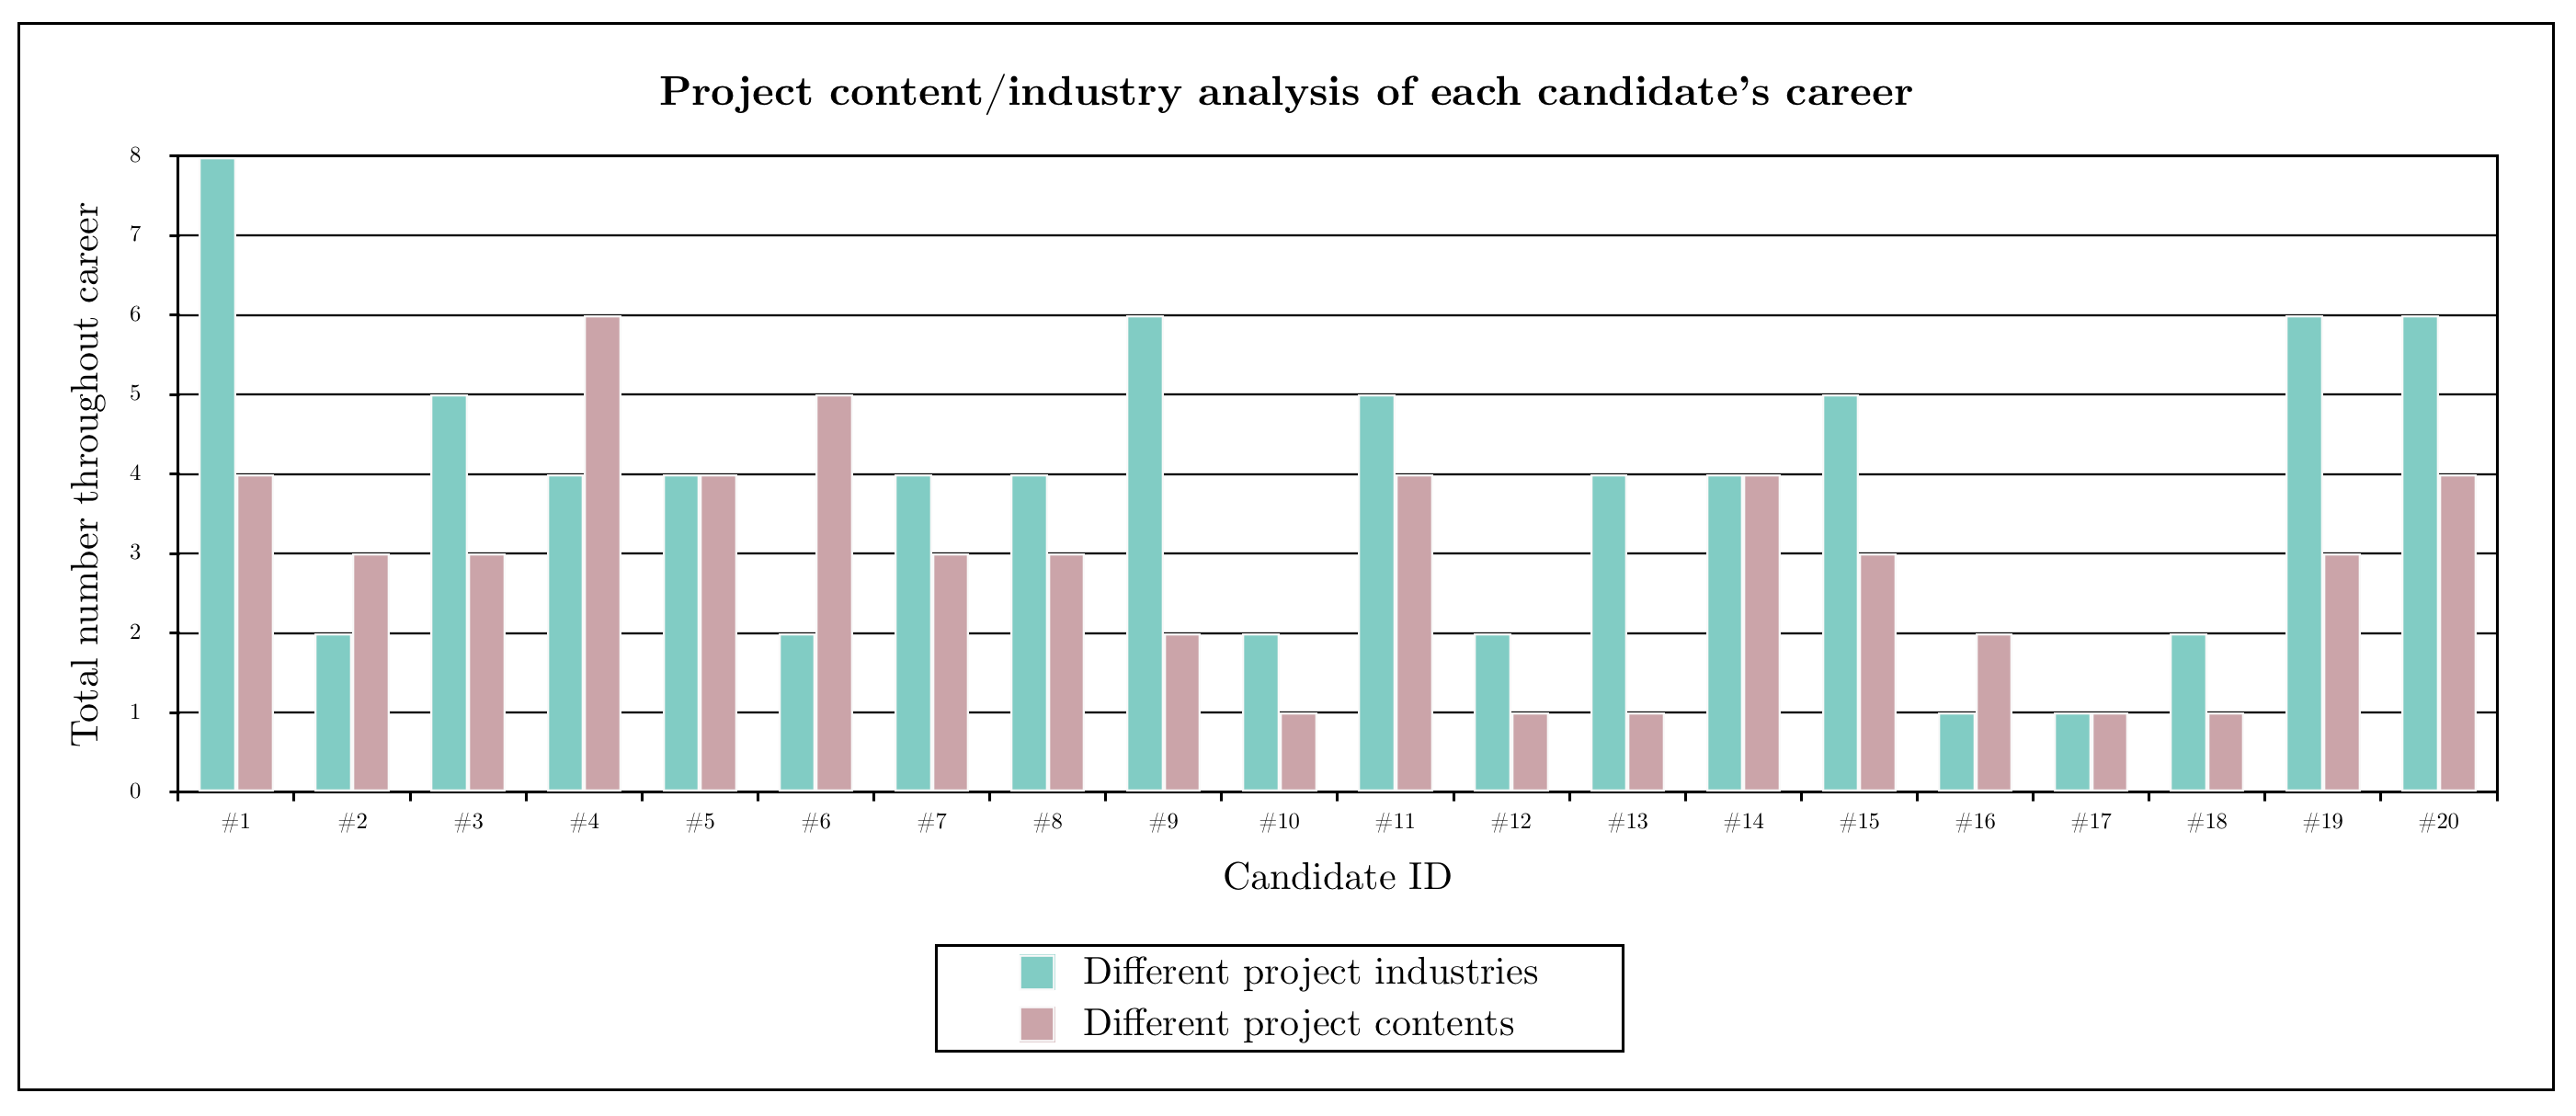
\includegraphics[width=1.0\columnwidth]{figures/Analysis_cand1.png}
  \caption[Analysis of distinct project contents and industries respectively the PP's career]{Analysis of the total number of distinct project contents and industries respectively the entire career of each project professional.}
  \label{fig:analy_cand1}
\end{figure}















%————————————————————–––––––Sub–Subsection–2————––––––––———————————————

\subsubsection{From the career movement model}

After already providing insights from various perspectives into the data sets in the previous subsection, this section takes the findings from the main working model and analyses them for changes or 'movements' during a project professional's career. To do so it uses the career movement model, which was introduced in detail on page \pageref{fig:alternate}f.  \\




%———————————————–––—————The–Individual–perspective—————––———————————

\noindent {\bf The individual career movements}\\[.1cm]
In the first step of this analysis stage, the movements in each project professional's career were visualised using the on page \pageref{sec:cmm}f introduced career movement model, which means for all 20 candidates of the sample group an individual graph was drawn up. These graphs can be seen in figures \ref{fig:CM1} and \ref{fig:CM2} on page \pageref{fig:CM1}f. The graphs are labeled with the candidate's ID on top, so that they can be easily allocated to each interviewee. This first comprehensive visualisation is aimed at facilitating the visual identification of patterns between individuals and furthermore was gives an overview over the careers with respect to project contents and project industries. For example, the graphs of project professionals of the same background, like \#16 and \#17 (both infrastructure industry) can be directly compared and, as can be seen in figure \ref{fig:CM2}, both do mostly projects with the same content and in one project industry. If these can be identified as patterns will be discussed in the following chapter.\\



%———————————————–––—————The–Sector–analysis—————––———————–––––––————

\noindent {\bf The sector analysis}\\[.1cm]
Since a comparative analysis of all the previously presented individual career movement analyses at once would be unfeasible by putting each interviewee's career movements into one graph, a sector classification model was developed, which can be seen in figure \ref{fig:sectors1} on page \pageref{fig:sectors1}. It divides the underlying model into 5 sectors. The sectors form and size was chosen considering not only the non-numeric scaling from one to many of the model, but also the underlying numeric scale, as well as the data sets. Thereby, all points covered by one of the sectors has an similar degree of career differentiation by project industries and project contents. The exact project content (PC) and industry (PI) combinations compromised by each sector are:
\begin{itemize}[noitemsep]
    \item Sector 1: one PC – one PI;
    \item Sector 2: one PC – two PI, two PC – two PI, two PC – one PI;
    \item Sector 3: one PC – three PI, two PC – three PI, three PC – three PI, three PC – two PI, three PC – one PI;
    \item Sector 4: one PC – four PI, two PC – four PI, three PC – four PI, four PC – four PI, four PC – three PI, four PC – two PI, four PC – one PI;
    \item Sector 5: one PC – five PI, two PC – five PI, three PC – five PI, four PC – five PI, five PC – five PI, five PC – four PI, five PC – three PI, five PC – two PI, five PC – one PI;
\end{itemize}
As a result, this enables the analysis and interpretation of the movements between these defined sectors of the entire sample group all at the same time. \\



\begin{figure}[hbt]
    \captionsetup{font=small}
  \centering
  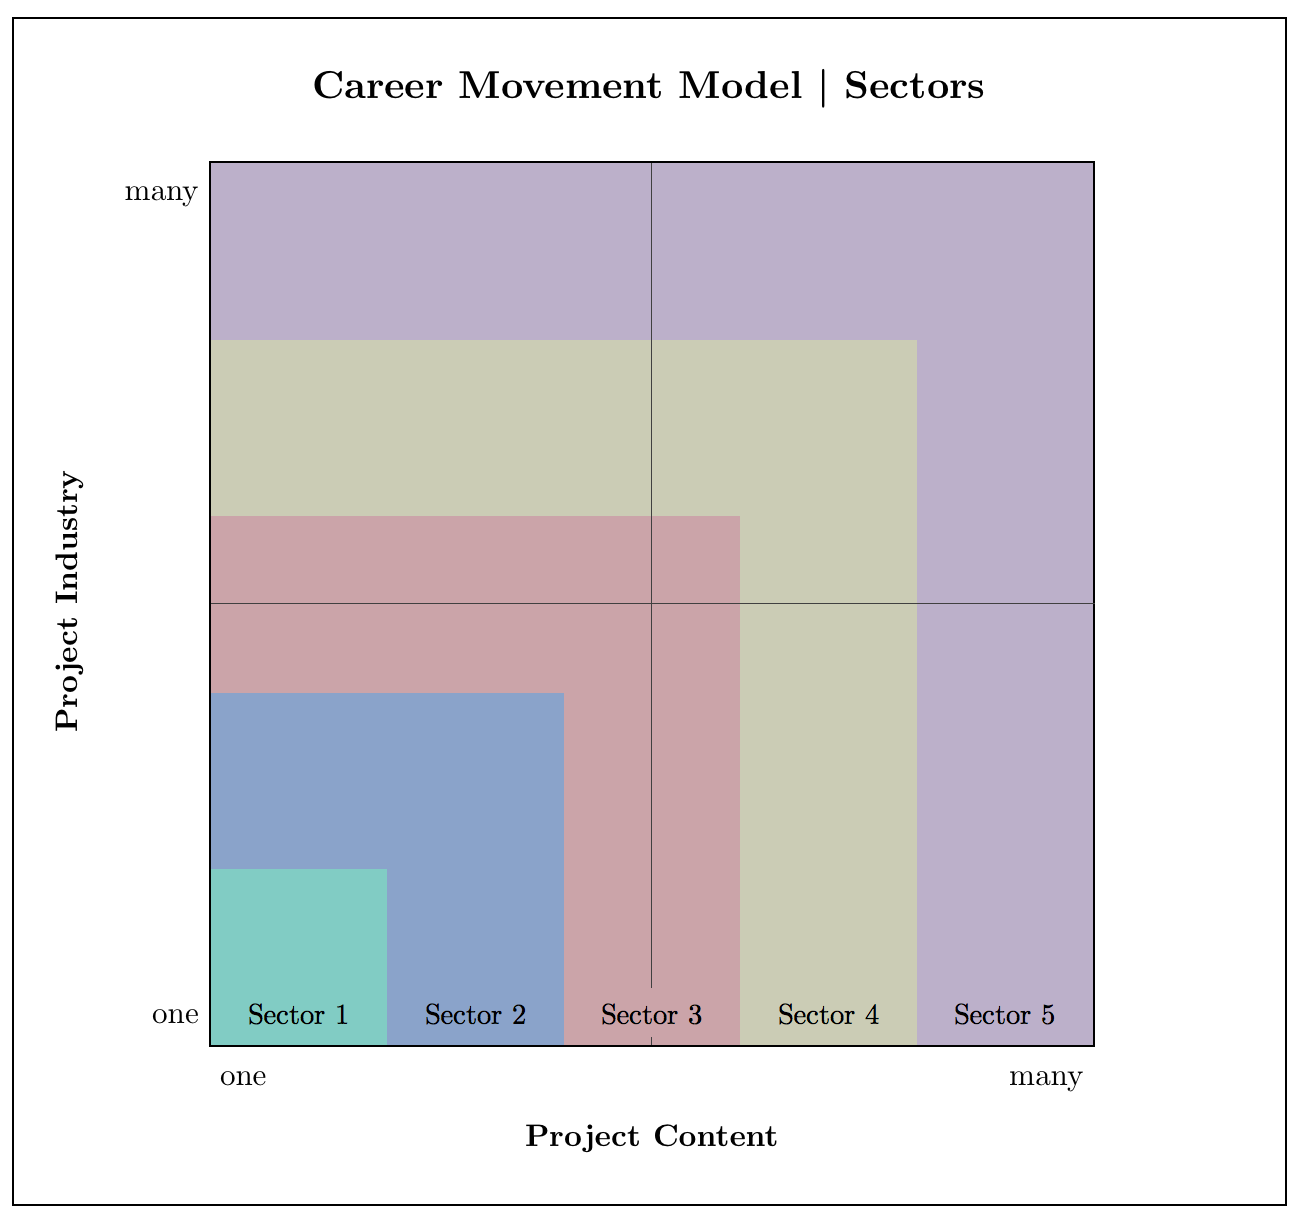
\includegraphics[width=.5\columnwidth]{figures/Analysis_sectors1.png}
  \caption[The sector classifications]{The sector classifications, which are to be used for the career movement model.}
  \label{fig:sectors1}
\end{figure}

\noindent Using this sectorisation, figure \ref{fig:sector2} (p. \pageref{fig:sector2}) shows the outcomes of the conducted sector analysis, which examined how much the bubbles located in a sector made up of the total number of bubbles for each term. Thereby it shows the percentage of project professionals that execute a similar number of different project contents and industries in each step of the career. As can be seen in figure \ref{fig:sector2}, in the first period of their career, 63\% of the project professionals work in project(s) with a maximum of 2 different project contents and/or industries and this trend continues in the second term as the percentage rises to 80\%. However, the first period is also the only one, where some (5\%) project professionals do projects with 5 distinct project contents and or industries. In the third career phase the biggest group (38\%) of project personnel does projects with only one project content and one project industry. The of located in sector 3 is increasing significantly from 7\% in period 2 to 23\%. This movement happens at the cost of sector 2 which falls significantly from 47\% in the \nth{2} term to 23\% in the \nth{3}. This trend further increases, as in the \nth{4} period the majority (46\%) of the sample group conducts projects with 3 project contents and/or industries. In this term none conduct projects in the \nth{4} sector. Sector 1 and 2 project combinations are done by 31\% and 23\%, respectively. In the last career period, however, the share of Sector 3-type project falls drastically to 14\%. Therefore, Sectors 1, 2 and 3 profit and rise again to 43\%, 29\% and 14\%, respectively. \\


\begin{figure}[hbt]
    \captionsetup{font=small}
  \centering
  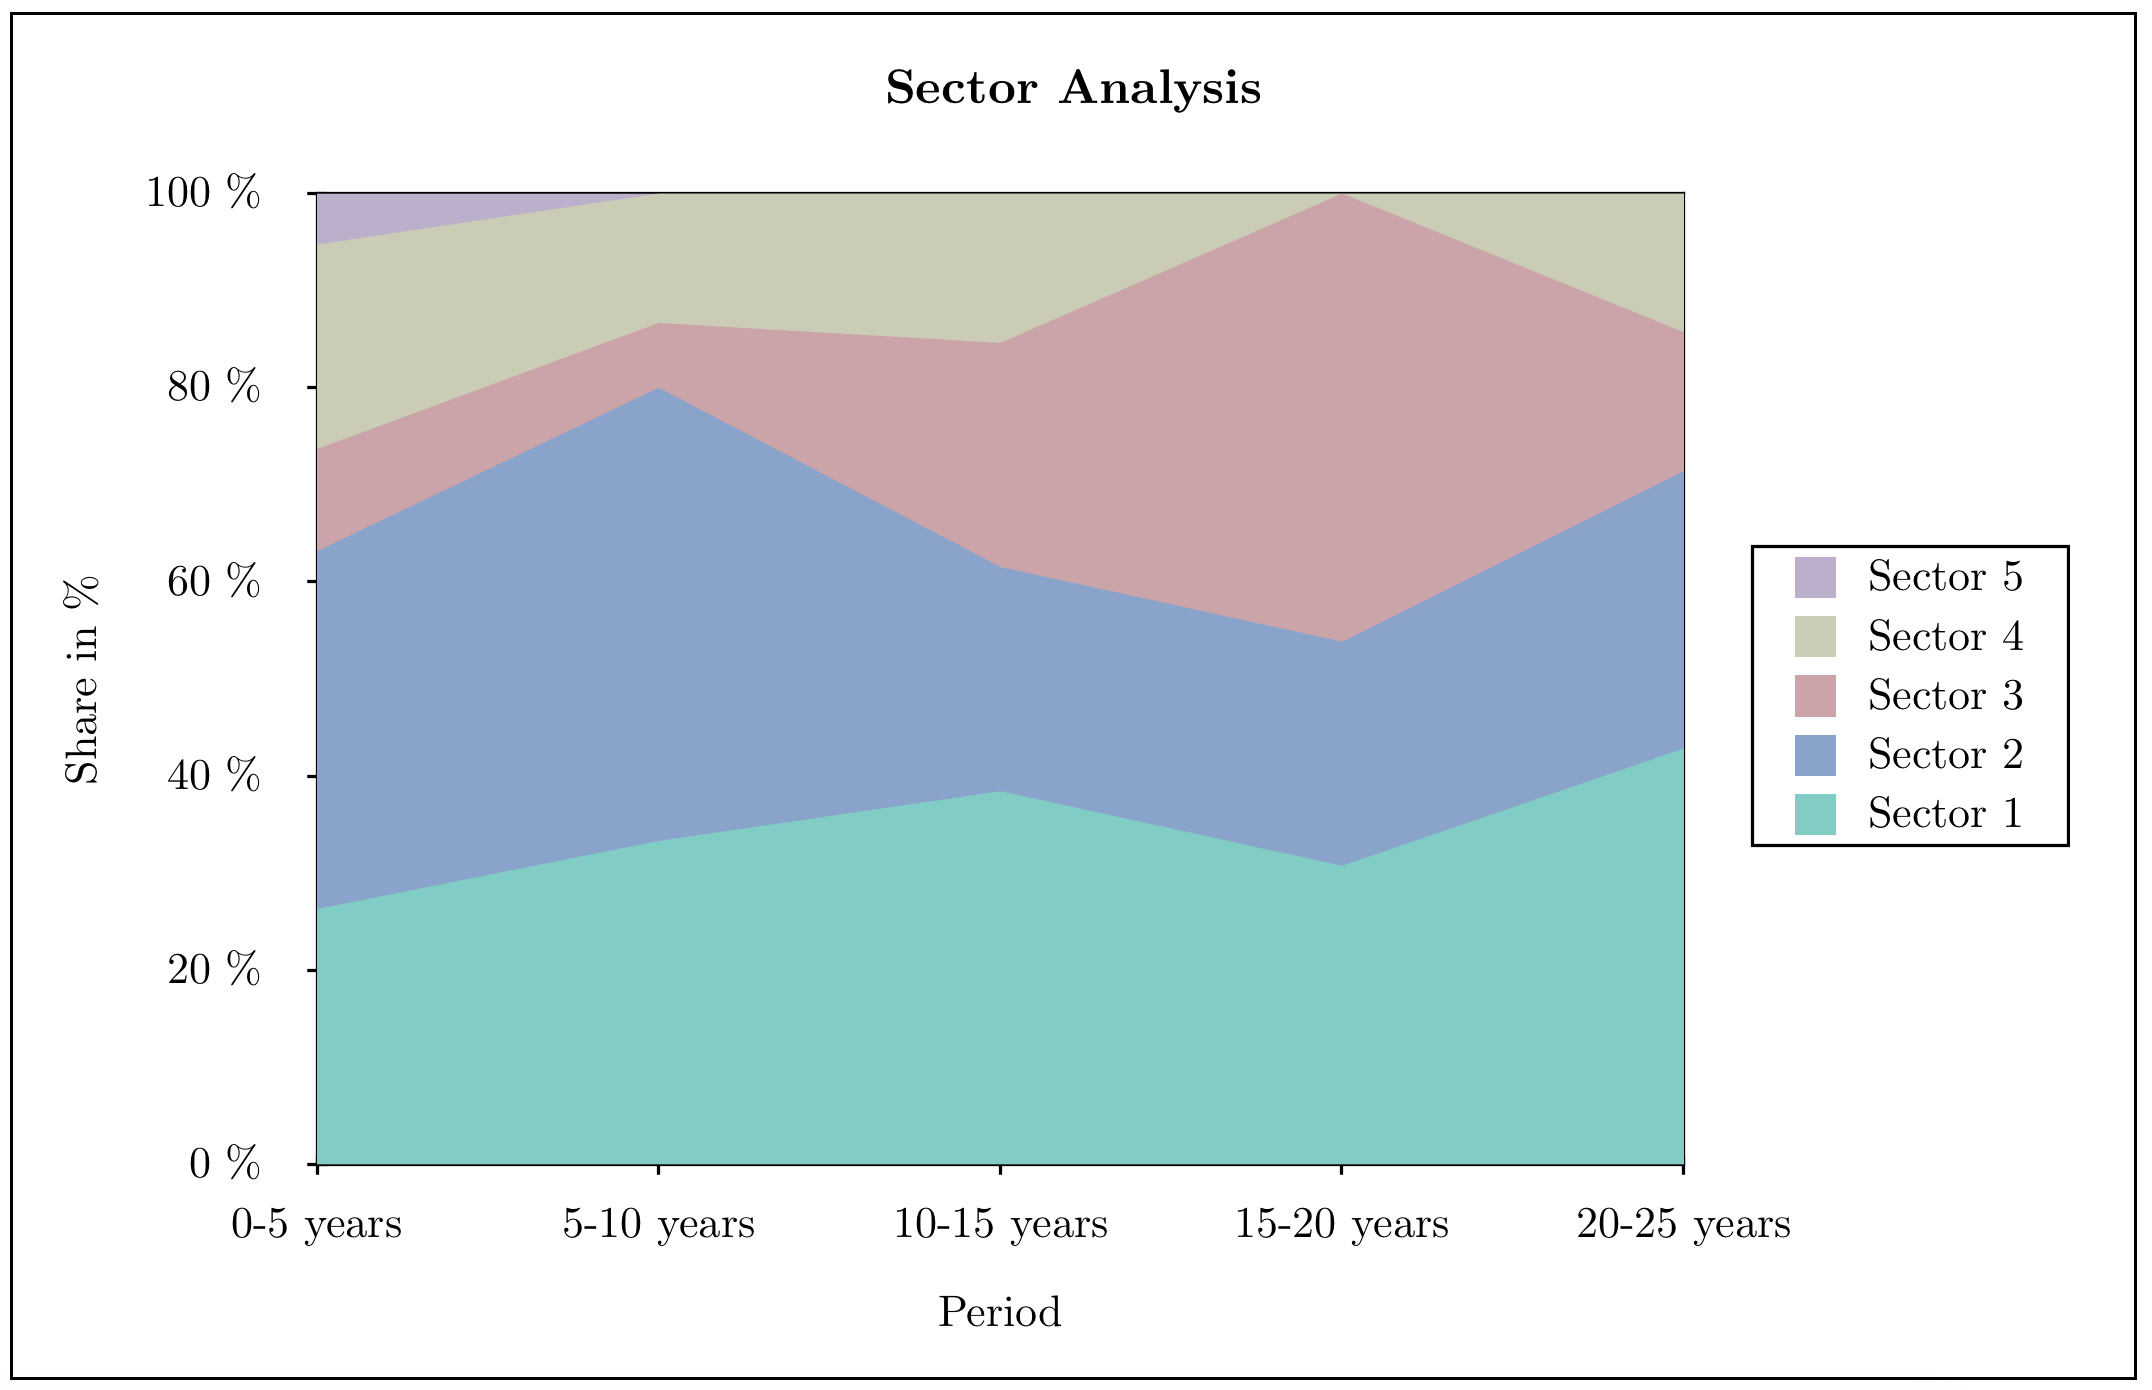
\includegraphics[width=.6\columnwidth]{figures/Analysis_sectors2.png}
  \caption[Results of the sector analysis]{Results of the sector analysis, showing the share of project professionals located in each of the five sector per career period.}
  \label{fig:sector2}
\end{figure}


\subsection{Summary of the study results}
In this chapter, the results of the study, as well as several conducted analyses were presented, which shed a light on the careers of project professionals from perspective. Firstly, it was shown, that the working model fulfils its purpose and delivers analysable results, but also can be applied to the careers of project professional of different backgrounds and form. Furthermore, the visualisation helps to identify pattern and interpret the data, as will be seen in the following chapter. Whether form these obtained findings,  patterns or other assumptions about the careers of project professional can be derived or not will be discussed in the following chapter.  \\

\begin{sidewaysfigure}[!hbt]
    \captionsetup{font=small}
  \centering
  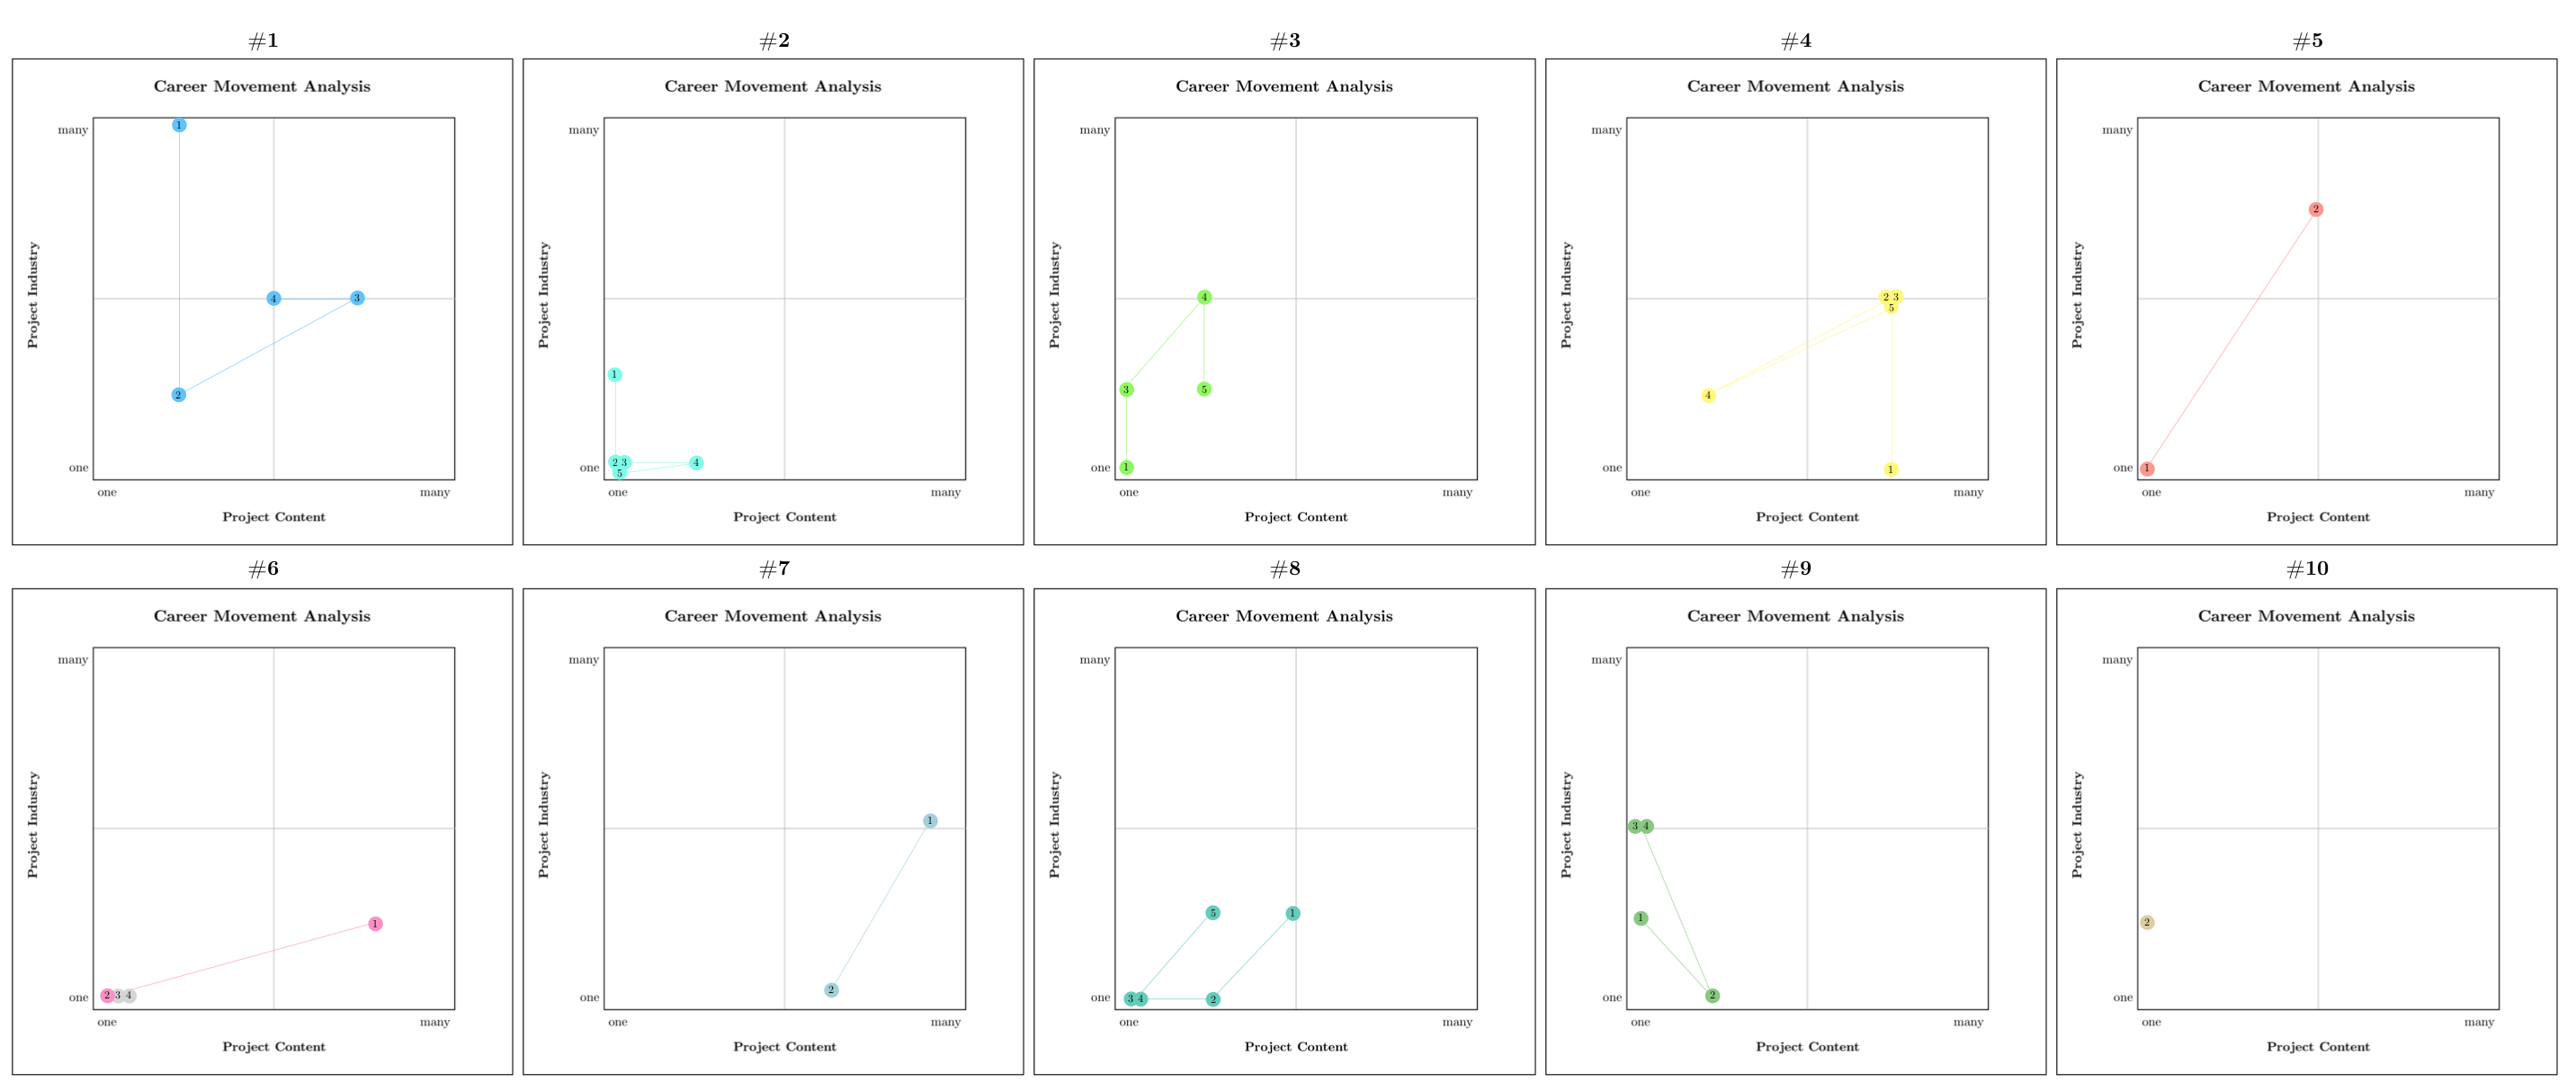
\includegraphics[width=1.0\columnwidth]{figures/Analysis_CM1.png}
  \caption[Results of the career movements model for each individual – Part I]{Results of the career movements model for each individual – Part I}
  \label{fig:CM1}
\end{sidewaysfigure}

\begin{sidewaysfigure}[!hbt]
    \captionsetup{font=small}
  \centering
  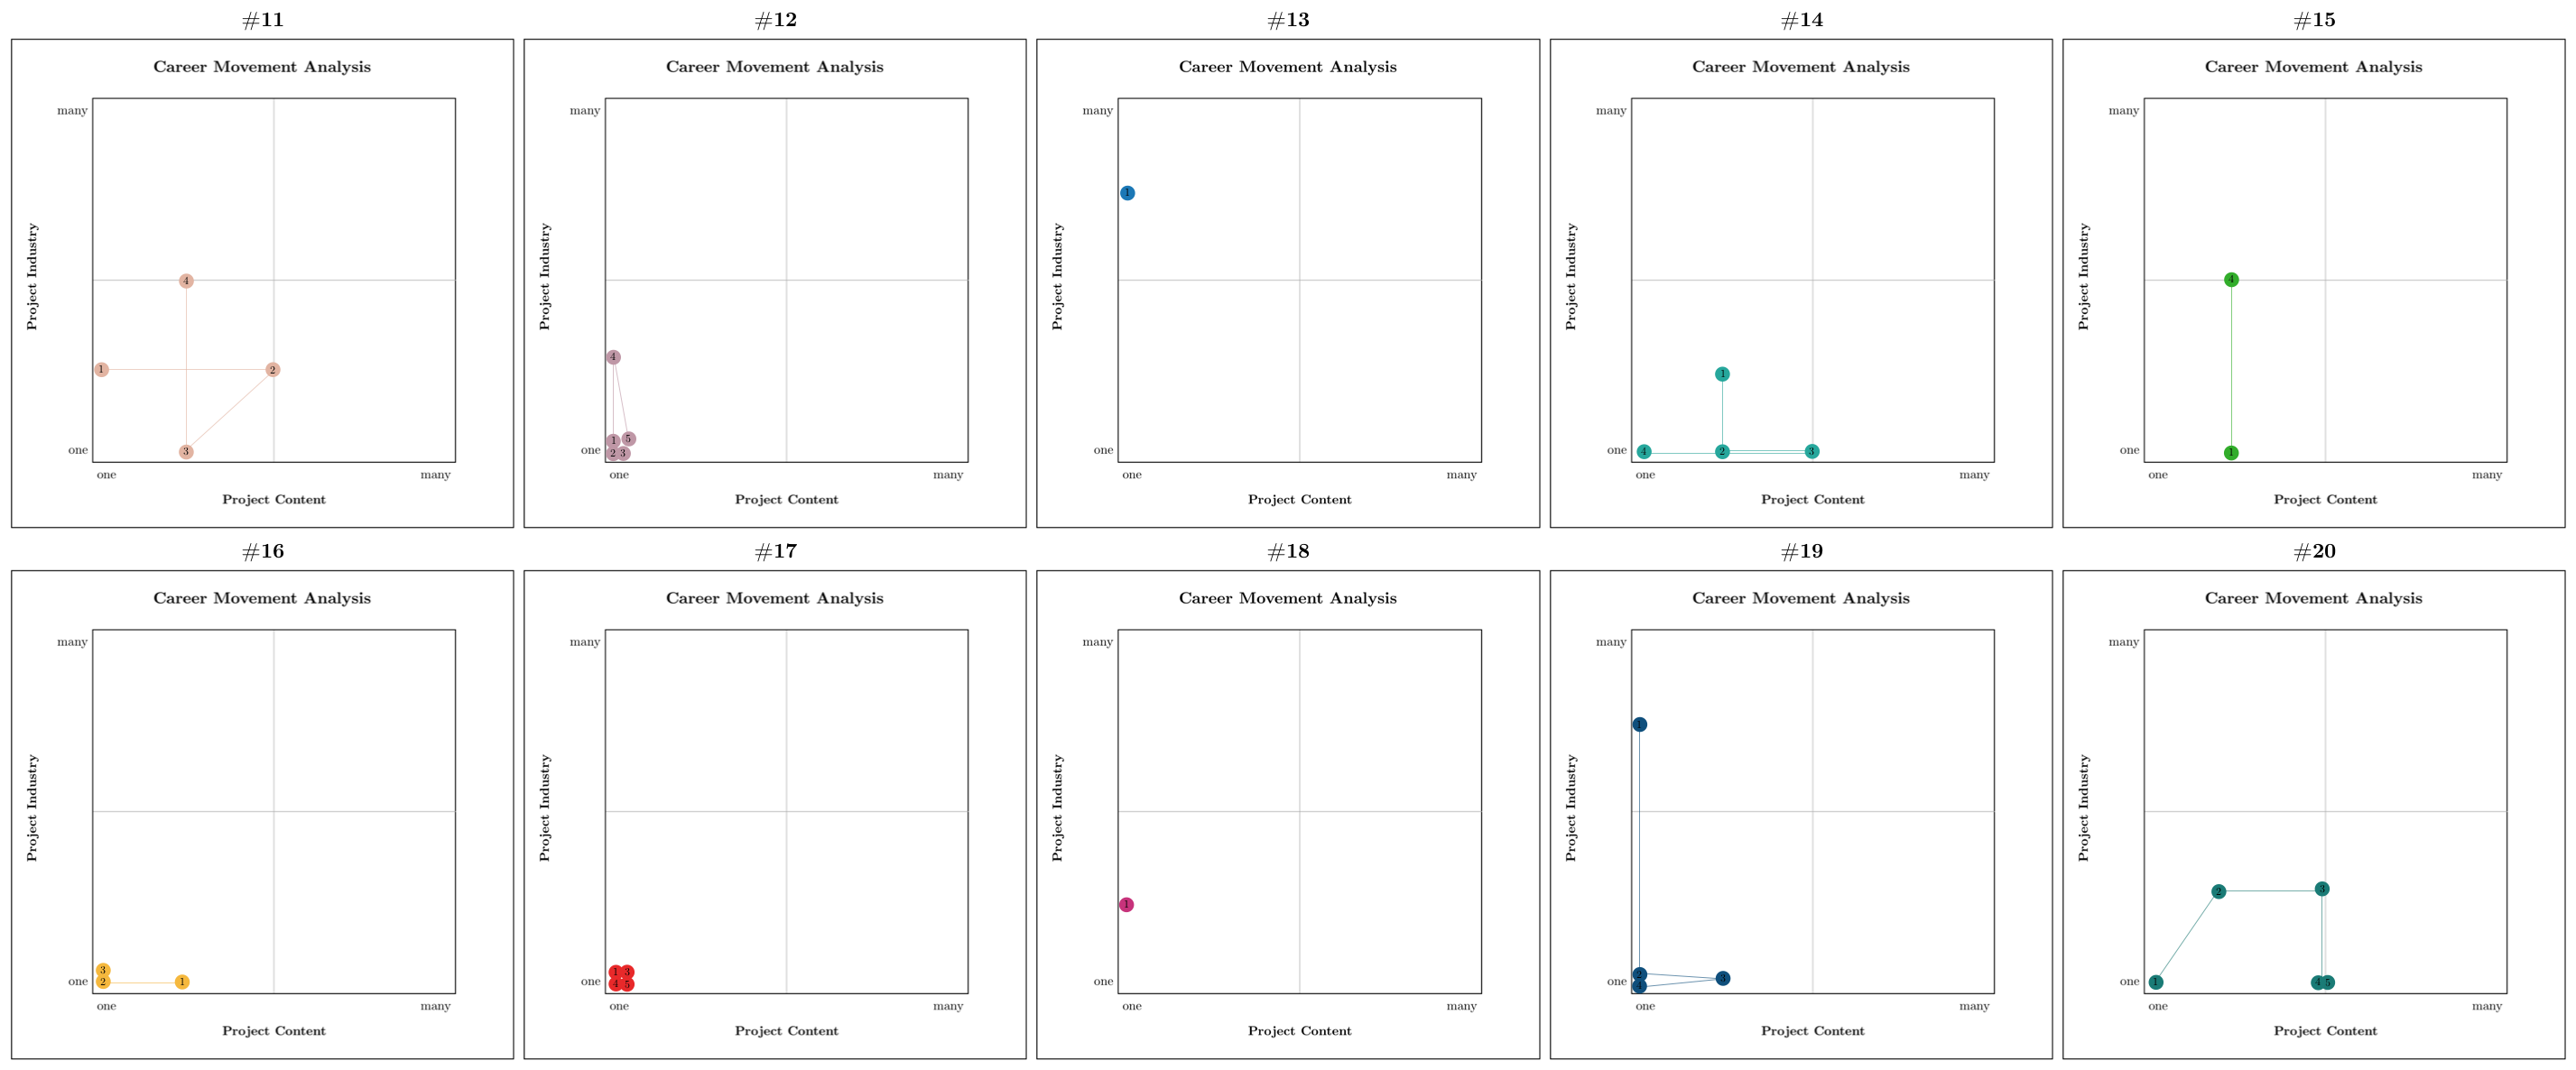
\includegraphics[width=1.0\columnwidth]{figures/Analysis_CM2.png}
  \caption[Results of the career movements model for each individual – Part II]{Results of the career movements model for each individual – Part II}
  \label{fig:CM2}
\end{sidewaysfigure}